\documentclass[a4paper,12pt]{article}

% ==================== 宏包加载 ====================
\usepackage{geometry}
\usepackage{xeCJK}
\usepackage{xltxtra}
\usepackage{titlesec}
\usepackage{tocloft}
\usepackage{fancyhdr}
\usepackage{setspace}
\usepackage{enumitem}
\usepackage{hyperref}
\hypersetup{
    colorlinks=false,
    pdfborder={0 0 0}
}
\usepackage{amsmath,amssymb}
\usepackage{booktabs}
\usepackage{multirow}
\usepackage{array}
\usepackage{threeparttable}
\usepackage{longtable}
\usepackage{graphicx}
\usepackage{float}
\usepackage{caption}
\usepackage{subcaption}
\usepackage{xcolor}
\usepackage{indentfirst}
\usepackage{etoolbox}

% ==================== 三线表配置 ====================
\setlength{\heavyrulewidth}{1.5pt}   % 顶线和底线粗细
\setlength{\lightrulewidth}{0.75pt}  % 栏目线粗细
\setlength{\cmidrulewidth}{0.4pt}    % \cmidrule 粗细
\newcommand{\doubleline}{\midrule[0.75pt]}  % 双竖细线（用于过宽表格分隔）

% ==================== 页面设置 ====================
\geometry{left=30mm, right=25mm, top=30mm, bottom=25mm}
\setlength{\headheight}{15pt}

% ==================== 字体设置 ====================
% 定义 CJK 字体族
\setCJKfamilyfont{zhwsong}{SimSun}
\setCJKfamilyfont{hei}{SimHei}
\setCJKmainfont{SimSun}[BoldFont=SimHei] 
\setmainfont{Times New Roman}[BoldFont=Times New Roman Bold]

\newcommand{\huawenzhongsong}{\CJKfamily{zhwsong}}
\newcommand{\heiti}{\CJKfamily{hei}}

% ==================== 字号定义 ====================
\newcommand{\xiaochu}{\fontsize{36}{46}\selectfont}
\newcommand{\erhao}{\fontsize{22}{30}\selectfont}
\newcommand{\xiaoer}{\fontsize{18}{24}\selectfont}
\newcommand{\sanhao}{\fontsize{16}{24}\selectfont}
\newcommand{\sihao}{\fontsize{14}{20}\selectfont}
\newcommand{\xiaosi}{\fontsize{12}{18}\selectfont}
\newcommand{\xiaosihao}{\fontsize{12}{18}\selectfont}
\newcommand{\wuhao}{\fontsize{10.5}{15}\selectfont}

% ==================== 行距设置 ====================
\renewcommand{\baselinestretch}{1.5}

% ==================== 图表标题格式 ====================
\DeclareCaptionFont{cnlabelfont}{\heiti\sihao\bfseries}
\DeclareCaptionFont{cntextfont}{\heiti\xiaosi}
\DeclareCaptionLabelSeparator{cncolon}{：}
\captionsetup[table]{labelsep=cncolon,labelfont=cnlabelfont,textfont=cntextfont}
\captionsetup[figure]{labelsep=cncolon,labelfont=cnlabelfont,textfont=cntextfont}
\renewcommand{\tablename}{表}
\renewcommand{\figurename}{图}

% ==================== 表格内容格式 ====================
\AtBeginEnvironment{table}{\xiaosi}
\AtBeginEnvironment{tabular}{\xiaosi}

% ==================== 封面页定制 ====================
\newcommand{\makeWHSCover}[6]{%
    \begin{titlepage}
        \centering
        \vspace*{1cm}
        
        {\huawenzhongsong\xiaochu\bfseries 武汉体育学院学士学位论文\par}
        
        \vspace{2cm}
        
        {\heiti\erhao\bfseries #1\par}
        
        \vspace{3cm}
        
        \hspace{2cm}
        \begin{minipage}{0.45\textwidth}
            \raggedright
            \huawenzhongsong\sanhao
            院\qquad 系：#2 \\[1em]
            专\qquad 业：#3 \\[1em]
            姓\qquad 名：#4 \\[1em]
            学\qquad 号：#5 \\[1em]
            指导教师：#6
        \end{minipage}
        
        \vfill
        
        {\huawenzhongsong\sanhao \the\year 年 \the\month 月\par}
    \end{titlepage}
    \clearpage
}

% ==================== 摘要及关键词定制 ====================
\newenvironment{abstractcn}{%
    \thispagestyle{empty}
    \begin{center}
        {\heiti\erhao\bfseries 摘\quad 要}
    \end{center}
    \vspace{1em}
    \par\huawenzhongsong\xiaosi\relax
}{%
    \par\vspace{2em}
    \noindent{\heiti\sihao\bfseries 关键词：}\huawenzhongsong\xiaosi
}

\newenvironment{abstracten}{%
    \thispagestyle{empty}
    \begin{center}
        {\heiti\erhao\bfseries ABSTRACT}
    \end{center}
    \vspace{1em}
    \par\xiaosi\relax
}{%
    \par\vspace{2em}
    \noindent{\heiti\sihao\bfseries Keywords:}\xiaosi
}

% ==================== 目录定制 ====================
% 目录设置在 \tableofcontents 之前立即执行
\newcommand{\setupContents}{%
\renewcommand{\contentsname}{\heiti\xiaoer\bfseries 目\quad 录}
\renewcommand{\cftsecfont}{\huawenzhongsong\xiaosi}
\renewcommand{\cftsubsecfont}{\huawenzhongsong\xiaosi}
\renewcommand{\cftdotsep}{4.5}
\renewcommand{\cftsecpagefont}{\normalfont\xiaosi}
}

% ==================== 正文标题格式 ====================
\setcounter{secnumdepth}{4}

\titlespacing*{\section}{0em}{1em}{1em}
\titlespacing*{\subsection}{0em}{1em}{1em}
\titlespacing*{\subsubsection}{0em}{1em}{1em}
\titlespacing*{\paragraph}{0em}{1em}{0em}

\setlength{\parindent}{2em}

% ==================== 列表环境定制 ====================
\setlist[enumerate,1]{label=(\arabic*), leftmargin=*, itemsep=0pt, parsep=0pt, topsep=0.5em}
\setlist[enumerate,2]{label=\textcircled{\small\arabic*}, leftmargin=*, itemsep=0pt, parsep=0pt, topsep=0.5em}

% ==================== 页眉页脚 ====================
\pagestyle{fancy}
\fancyhf{}
\fancyfoot[C]{\thepage}
\renewcommand{\headrulewidth}{0pt}
\renewcommand{\footrulewidth}{0pt}

\begin{document}

% ==================== 封面 ====================
\makeWHSCover{HIIT 对舞蹈啦啦操运动员专项技术动作提升的实验研究}{艺术学院}{舞蹈表演}{王语桐}{2022331464}{李洪波}


% ==================== 目录 ====================
\cleardoublepage
\pagenumbering{Roman}
\setupContents
\tableofcontents
\cleardoublepage

% ==================== 中文摘要 ====================
\begin{abstractcn}
	本研究探究为期6周的专项高强度间歇训练对舞蹈啦啦操运动员技术动作的影响，验证专项HIIT相较于传统间歇跑训练的优势。采用随机对照实验设计，将20名女大学生舞蹈啦啦操运动员随机分为实验组和对照组各10人。实验组进行专项HIIT训练，对照组进行400米间歇跑，两组训练周期均为6周。测试指标包括屈体分腿跳腾空高度、双腿开度、阿拉C杠转体位移距离、技术动作衰减率、心率恢复率和主观疲劳度。

	干预后，实验组疲劳状态下腾空高度衰减率从16.8\%降至8.5\%，双腿开度衰减率从7.0\%降至3.3\%，阿拉C杠转体位移距离从42.3 cm降至28.5 cm，均显著优于对照组。实验组心率恢复率显著提升，主观疲劳度显著降低。相关性分析显示，心率恢复率改善与腾空高度衰减率呈显著负相关。结果表明，专项HIIT训练能够显著降低舞蹈啦啦操运动员在疲劳状态下的技术动作衰减率，有效提升抗疲劳爆发力和核心控制稳定性，验证了专项特异性适应原则在难美项群体能训练中的应用价值。
\end{abstractcn}
舞蹈啦啦操，专项HIIT，技术动作衰减率，抗疲劳爆发力，SAID原则

% ==================== 英文摘要 ====================
\cleardoublepage
\begin{abstracten}
	This study investigated the effects of a 6-week sport-specific high-intensity interval training program on technical performance in dance cheerleading athletes. A randomized controlled trial was conducted with 20 female collegiate dance cheerleading athletes randomly assigned to an experimental group receiving sport-specific HIIT or a control group performing 400m interval running. Both groups trained for 6 weeks. Outcome measures included jump height, leg angle, displacement distance during C-bar turns, technique decay rate, heart rate recovery, and rating of perceived exertion.

	Post-intervention, the experimental group showed significant reductions in jump height decay rate from 16.8\% to 8.5\%, leg angle decay rate from 7.0\% to 3.3\%, and turn displacement distance from 42.3 cm to 28.5 cm, all significantly better than the control group. Heart rate recovery significantly improved and perceived exertion significantly decreased in the experimental group. Correlation analysis revealed a significant negative correlation between heart rate recovery improvement and jump height decay rate. The results indicate that sport-specific HIIT can significantly reduce technique decay rate in dance cheerleading athletes under fatigue, effectively improving fatigue-resistant explosive power and core control stability, validating the application of the Specific Adaptation to Imposed Demands principle in aesthetic sports training.
\end{abstracten}
dance cheerleading, sport-specific HIIT, technique decay rate, fatigue-resistant explosive power, SAID principle

% ==================== 正文 ====================
\cleardoublepage
\pagenumbering{arabic}
\setcounter{page}{1}

\section{引言}

\subsection{研究背景}
舞蹈啦啦操，这一项目无论是在国内还是在国外，都正在以难以想象的速度快速发展，因此这一项目所体现的竞技水平也在飞速提升。
如今，舞蹈啦啦操对运动员的 专项技术能力要求也在日益提高。在我国，舞蹈啦啦操自2000年左右被引入后也发展迅猛，
迄今为止，这一项目已然形成了从青少年培训到高等院校专业人才培养的完整体系。根据滕思佳的研究，舞蹈啦啦操属于技能主导类表现难
美性项群\cite{teng2012}，，其项目特征在于通过高规
格的技术动作和优美的艺术表现来获得裁判的评分，从而进行竞争排名。

依据国际啦啦操联合会（ICU）2025版竞赛规则\cite{icu2025}，舞蹈啦啦操
项目的成套动作时长被严格限定在2分15秒至2分30秒之间。
成套动作的编排需涵盖爆发性技术、控制性技术以及表现性技术这三类核心技术要素。
除此之外，成套动作还要求运动员展示精确的队形变化、流畅的空间调度以及与音乐节奏的高度契合。
对于成套动作的评分体系涵盖了技术完成分、艺术表现分和综合印象分等多项分数，对运动员的综合素质提出了非常高的能力要求。
如果我们从运动生理学的视角对舞蹈啦啦操表演成套动作的过程进行能量代谢分析，这一过程属于比较典型的次极限强度运动。
在表演成套动作的过程中，糖酵解供能系统在总的能量供应中，占比大概是60\%到70\%。在成套动作结束之后，运动员
的血乳酸浓可以达到8-12 mmol/L。

在如此高的能量消耗下，也会随之出现一些问题，例如随着竞技强度的提升，运动员在比赛的后半程普遍会出现技术动作展示不完美、不充
分的情况。运动员极易出现如腾空高度
降低、双腿开度不
足、转体重心偏移、手位发
力拖沓等代偿动作。

舞蹈啦啦操核
心技术动作可分
为爆发性技术、控制性技
术和表现性技术三类。屈体分
腿跳作为爆发性技术的代表，要
求腾空高度充分且双腿完全伸直；
阿拉C杠转体作为控制性技术的代表
，要求核心极度稳定且动力腿不掉
高度；手位组合作为表现性技术的
代表，要求胸挺收腹、肩锁臀夹，
手位变换准确、快速、有力，并与
音乐节奏、队形变化高度契合。

因此，如何在疲劳状态下去维持这些技术动作的稳定性，成为了舞蹈啦啦操训练最核心的问题之一。

高强度间歇训练（High-Intensity Interval Training, HIIT）是一种高效、新型的
训练模式。
这一训练模式的独特价值在于，其能够精准地去模拟比赛中的能量代谢供能模式。
如果我们结合
专项动作的特征针对性地进行设计HIIT方案，则能够让寻动员在比赛时高效地募集更多肌纤维，尤
其是快肌纤维。这样的结果对于维持爆发性技术动作的高质量完成通常具有决定性的意义。同时，这为
舞蹈啦啦操项目的训练模式的优化提供了重要的理论依据和实践方向。

\subsection{研究意义}

在先前的研究背景之下，本研究具有重要的理论意义和实践意义。

一是在理论层面，本研究验证了专项特异性适应原则（SAID原则）在难美项群体能训练中的重要应用价值。现有研究很多都是
关注一般性的体能训练 或者是 单一运动项目的HIIT效果，较少又研究将专项技术动作直接融入进高强度间歇训练进行的系统探究。
本研究通过对比专项HIIT与传统间歇跑的训练效果，验证了
"专项动作诱导专项适应"的理论假设，为难美项群专项体能训练理论提供了实证支持。

二是在实践层面，本研究为舞蹈啦啦操训练模式的优化提供了科学依据。当前多数队伍的训
练体系中普遍存在着体能训练与技术表现脱节的问题。有相当数量的运动
队仍然在沿用长距离慢跑或者是单一形式的间歇跑作为主要的体能训练手段。然而本研
究通过实验验证，为基层教练员在训练实践中选择更具专项针对性的体能训练方法提供了参考。这有助于
将运动员的体能储备更高效地转化为竞技技术表现。


\subsection{研究现状}

接下来我们将从国内外的研究现状出发，对本实验的研究方向进行探究。
我们知道，无论是在比赛过程中还是在训练过程中，运动疲劳均会导致以下两个关键问题。
其中之一是大脑发出的动作指令运动员难以精准执行，
另外是肌肉的发力速度和力量输出功率会显著地下降。
Gandevia的研究指出，在运动生理学层面，肌肉疲劳涉到及中枢以及外周两个层
面的相互作用\cite{gandevia2001}。中枢层面表现
为大脑对肌肉的控制效率降低，外周层面则表现为肌肉本身的收缩能力下降。这正符合我们对运动疲劳产生的影响的直觉。
魏佳琳等进一步研究发现，疲劳状态下运动员单腿落地时的神经肌肉控制策略会发生显著改变，落地的稳定性
明显降低，下肢关节的协调配合能力也减弱\cite{weijialin2023}。这一研究发现与舞蹈啦啦操运动员在成套动作后半程出
现的技术崩塌现象高度吻合。

在高强度间歇训练方面，Gibala等的系统综述指出，低容量HIIT可诱导线粒体生物
合成和氧化酶活性提升\cite{gibala2012}。陈伟和曹洁发现，HIIT可改善高水平现代五项运动员的力量和爆
发力表现\cite{chen2021}。Strepp等研究发现，7天HIIT冲击微周期可快速提升耐力运动员的峰值功率输出
和计时赛成绩\cite{strepp2024}。然而，上述研究多关注静息状态下的体能指标改善，较少涉及疲劳状态下技术动作稳定性的维持。

在啦啦操专项体能训练研究方面，已有研究发现专项体能训练可改善啦啦操运动员技术表
现，但其采用的是传统专项体能训练模式，如核心力量结合爆发力练习，改善幅度约为15-20\%。现有文献
多关注损伤预防或一般体能发展，较少将专项技术动作融入高强度间歇训练进行系统探究。

综上所述，现有研究存在以下不足：第一，多数HIIT研究关注一般性体能指标，缺乏对
专项技术动作在疲劳状态下表现的关注；第二，啦啦操专项体能训练研究多采用传统模式，训练效率有待
提升；第三，缺乏专项HIIT与传统体能训练的对比研究。基于此，本研究提出专项HIIT训练方案，探究其对舞蹈啦啦操运动员技术
动作的影响效果。

\subsection{研究目的}

本研究旨在探究为期6周的专项HIIT训练对舞蹈啦啦操运动员技术动作的影响，同时验证专项HIIT相较于传统间歇跑训练的优势。

本研究假设在进行为期6周的专项HIIT训练后，舞蹈
啦啦操运动员在疲劳状态下的技术动作衰减率能够显著降低，且专项HIIT训练的干预效果将会优于传统间歇跑的训练模式。

本实验的研究技术路线将包括三个阶段。在第一阶段，通过文献调研和预实
验确定测试指标和训练方案；随后第二阶段，本实验将实施6周随机对照干预，严格控制
训练质量和测试条件；在最后阶段，采用多种统计方法分析数据，探讨指标间的相关关系。


\section{研究对象与方法}

\subsection{研究对象}

本研究以武汉体育学院艺术学院舞蹈啦啦操院队的 20 名女大学生运动员作为实验对象。
所有受试者均需严格符合身体健康且无严重心血管疾病史，近6个月内无下肢骨骼肌肉损伤病史的纳入标准，并具备熟
练完成屈体分腿跳和阿拉C
杠等高难度技术动作的能力，且在实验期间未服用任何可能影响运动表现的药物或营养补充剂。

为了确保受试者在技术基础层面差异在实验允许的范围之内，本研究规定受试者需连续完成 3 次双腿开度达到 180°的屈
体分腿跳，并且在主力腿位移小于 20 cm 的
前提下连续完成至少 2 个 8 拍的阿拉 C 杠转体，以此要求作为量化技术
门槛。在参与基线水平评估的 24 名初筛运动员中，分别有 2 名运动员因存在陈旧
性下肢损伤和技术动作未达标而未能符合纳入标准，因此在排除这 4 人后，最终有 20 名受试者进入正式实验阶段。


本研究采用 S 形随机分组法，将受试者分配至每组各 10 人的实验组与对照组。这批年
龄在 19 至 22 岁、身高 160 至 170 cm、体重 48 至 58 kg 且训练年限为 2 至 5 年
的受试者，在两组间基本情况的 P 值检验中均大于 0.05，表明组间无显著差异且具有可比性。

\subsection{实验法}

本研究采用随机对照实验设计，对受试者实施双盲
评估。具体实现为均不让受试者与测试结果的分析人员了解到具体的分组意图，对分组意图进行保密。本研究将训练内容嵌
入到受试者的常规专项训练课程中，实验组与对照组在热身活动、柔韧素质练习、成套动作教学等
环节需要保持完全一致。具体的差别仅在核心体能干预模块采用不同训练方案，以此达到控制实验变量的目的。

如图\ref{fig:experiment-flow}所示，实
验流程涵盖了包括从基线测试到随机分组，随后6 周干预实施以及终期测试等各个阶段。
在实验进行的过程中，本研究实施了非常严格的质量控制措施，从而确保训练强度监控和测试条件的一致性，
以此能够最大限度地减少无关变量对实验结果的干扰。

\begin{figure}[H]
	\centering
	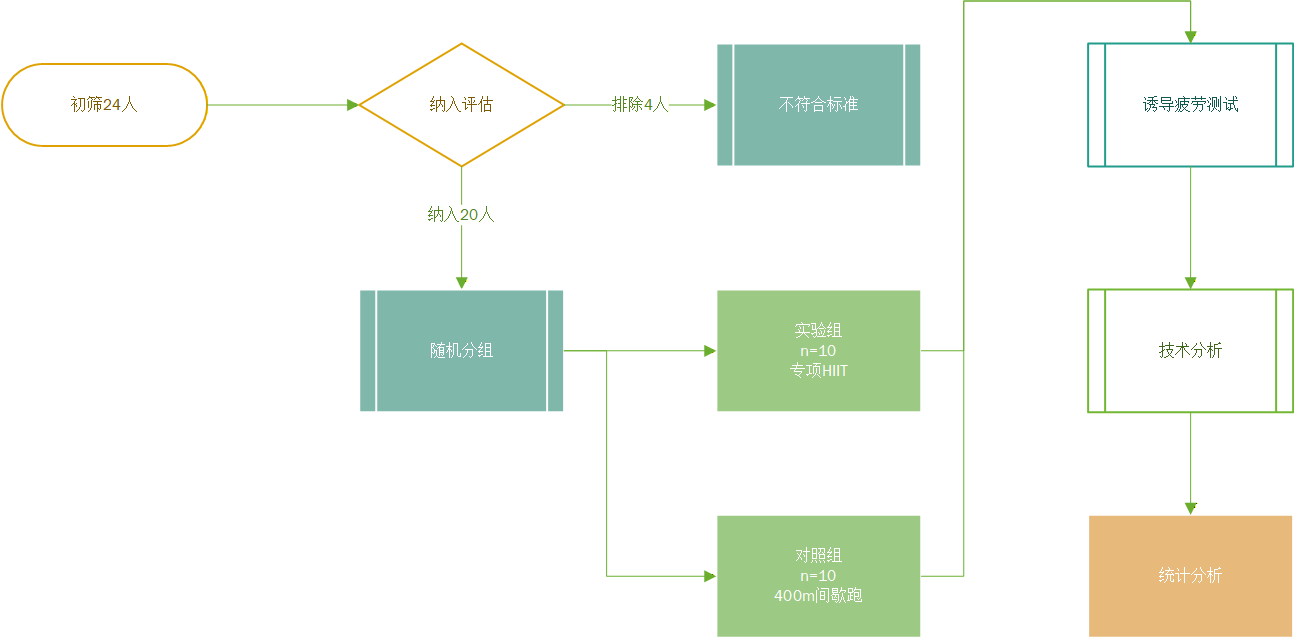
\includegraphics[width=\textwidth]{figures/placeholder-figure-1.png}
	\caption{实验流程图}
	\label{fig:experiment-flow}
\end{figure}

实验组采用专项 HIIT 训练方案，
具体为 Tabata 变式训练模式。专项HIIT训练方案的训练内容包括高抬腿 5 秒、
连续屈体分腿跳 5 次、波比跳 5 次、快速
开合跳 10 秒的循环组合。受试者需要全力完成 30 秒的高
强度运动之后进行 30 秒的间歇恢复，从而使运动与间歇的时间比为 1:1。受试者需要共计完
成 8 至 10 组这样的循环。本实验的强度监控主要采取心率监控，要求受试者的心率达到 170 次/分以
上，以 85\%至 90\%最大速度为参考。该方案的核心设计理念在于强
制要求运动员在心率极高的生理状态下依然能够高质量地输出专项技术动作
，借此强化神经肌肉系统对技术动作模式的控制与定型。

对照组采用一般间歇跑训练方案，具体为 400 米间歇跑。强度监控方面也以
心率为主，要求心率达到 170 次/分以上，以 85\%至 90\%最大速度
为参考，和实验组保持一致。间歇时间与跑动的时间比为 1:1，共计完成 6 至 8 组。
该方案旨在保持与实验组相近的生理负荷水平，但剥离了专项技术动作元素
，仅作为单纯的能量代谢训练对照，以验证\textquotedblleft 动作
模式特异性\textquotedblright 对技术提升贡献。

两组训练周期均为 6 周，每周 3 次，隔天进行。训练全程使用 Polar H
10 心率表进行实时心率监控，从而确保训练强度符合研究预设的标准。

\subsection{测试法}

本研究的核心关注点在于在疲劳状态下运动员专项技术动作的表现变化情况。针对这种变化情况的观测，测试法不失为一种非常优秀且科学
的方法，我采用了 疲劳诱导 结合 即刻技术测
试 的测试模式对受试者进行干预。

整体研究的完整测试流程
包含以下四个有序步骤。实验开始会进行 10 分钟的标准化热身活动，随后受试者需要进行休息至完全恢复，
在完全恢复的状态下完成屈体分腿跳和阿拉 C 杠转体的专项动作测试
，同时我记录静息状态下各受试者的基准数据。在完成基准测试之后，受试者需要全速完成一套标准的
2 分 30 秒成套动作。该完成过程要求心率至少达到 170 次/分以上，从而实现对比赛强度的模拟，以诱
导出受试者的生理疲劳状况。为了能够捕捉到受试者在疲劳状态下的技术表现情况，在完成成套动作后，受试者需要在 30 秒钟内立即完成屈体分
腿跳和阿拉 C 杠转体的转向动作测试。

对于转向动作的测试，我也设计了相应的指标对动作完成的情况进行科学化的量化，以便后续实验复现以及提升本研究的科学性与客观性。
我所设计的测试指标体系分为爆发性技术、控制性技术及辅助生理指标这三大类别。
爆发性技术指标指屈体分腿跳腾空的峰值高度和双腿开度。针对这两个指标，我均使用 Kinovea 运动视频
分析软件进行的测量工作，其中腾空高度通过对受试者髋部最高点进行标记，追踪这个标点的垂直位移即可获得。受试者的双腿开度指标直接
使用该软件的量角器功能进行测量。控制性技术指标包括阿拉 C 杠转体的重心位移距离和
有效完成圈数。针对前者，在记录的受试者转体的视频中，根据受试者的身高标记标准距离，再利用地面标记尺测量起止点直线距离，
从而得到真实的位移距离。
后者则直接采用人工计数记录。
最后一项指标，辅助生理指标包括运动后 1 分钟心率恢复值和主观疲劳度。详细地说HRR 是指运动结束后 1 分钟内心率
下降的数值，可以用于评估心肺功能恢复能力。RPE则是主观疲劳度， 采用 Borg量表进行记录
，该量表的打分制度设计为6至20分值，通过受试者主观对自身的疲劳程度进行打分
，打的分数越高表示受试者本身的疲劳感越强。

\subsection{数理统计法}

针对受试者专项技术动作表现所采集的原始数据，本研
究采用数理统计法对实验数据进行挖掘以及系统性的分析，采用 SPSS 26.0 统计软件进行数据处理与分析，所有计量资料统一采用均值加减标准差的形式进行呈现，用$\bar{x}\pm s$表示。

由于只有在数据服从正态分布时，使用参
数检验$t$检验得出的结论才是有效的，所以在进行统计之前，我对受试者相关数据进行了正态性检验，
以判断是否满足参数检验的前提假设。

本研究的采用的正态性检验的方法是 Shapiro-Wilk 法 \cite{li2009} ，该方法是目前针对小样本（$n<50$）最经常使
用的方法之一。相比于其他正态性检验方法例如 Kolmogorov-Smirnov 检验，Shapiro-Wilk 法在小样本条件
下具有更准确的检验结果。其检验结果以 $W$ 统计量和 $P$ 值的形式呈现，其中 $W$ 统计量的取值
范围为 0 至 1，如果数值越接近 1 则表示数据越接近正态分布。当 $P>0.05$ 时，可认为数据服从正态分布，满足使用 $t$ 检验等
参数统计方法的前提条件。在本研究中，受限于我所在的实验环境，暂时无法召集大批量的受试者进行试验研究，
所以采用这个正态性检验的方法极为合适。

考虑到本实验中同一受试者需要经历干预前后的重复测试，单纯的均值对比容易被个体基线体能的差异所掩盖。
为此，组内指标的纵向评估选定了配对样本 $t$ 检验。该方法的原理是比较配对样
本均值差异与零的差异是否具有统计学意义\cite{ma2017}。在本实验中，每位受试者在干预前后均接受了相同指标的测试，
因此配对样本 $t$ 检验能够有效
控制个体差异对结果的影响，更为精确地反映干预的效果，
从而提高检验的灵敏度。
至于专项 HIIT 训练究竟能否拉开不同组别之间的运动表现差距，则由独立样本 $t$ 检验来判定\cite{shen2007}。

针对各项实验指标，我引入了 Pearson 相关性分析 。这一统计手段主要考察两组数据
在 $-1$ 至 $+1$ 范围内的相关性关系\cite{sun2018}。
具体而言，$r$ 的正负值定义了相关性的方向，如果为正值，则是正相关。举个例子，规律且适量的运动越多，入睡越快，深度睡眠时间通常也
越长。那么运动的规律性和运动量于入睡速度以及睡眠深度就叫正相关，那么负相关也自然容易理解了。
而这个值的大小则直接对应了关联的强弱，
如果数据越接近 1 则意味着两者之间的关系越强。
通过这一方法，本研究能够深度揭示受试者心率恢复与技术衰减、疲劳感以及位移表现等指标间之间的相关性关系，
为后续阐述干预方案的影响机制也奠定了基础。

在本研究中，显著性水平设定为 $\alpha=0.05$，即当 $P<0.05$ 时认为差异具有统计学意义，当 $P<0.01$ 时认为差异具有高度
统计学意义。0.05 的显著性水平是医学和生物学研究领域约定俗成的标准，当 $P<0.05$ 时，我们有理由认为样本所代
表的总体之间存在真实差异。



\subsection{实验质量控制}

本研究实施了多维度的严格质量控制措施，就是为了确保实验结果的可靠性、有效性和可重复性。

我利用随机数字表法对受试者进行分组，由非实验人员制作密封信封进行分组分配，确保受试者分配的随机性和不可预测性。
参与分组的受试者仅被告知参与不同类型的体能训练研究，不清楚具体研究假设和预计效果。这样能够减少受试者心理因素对测
试结果的干扰。

针对关键测量指标，我进行了预实验检验。测试前对两名测评人员进行统一培训和一致性检验。
检验结果显示，腾空高度、双腿开度和位移距离的测试者间信度系
数分别为0.962、0.948和0.975，均大于0.90的可接受标准，表明两名测评人员的测量结果具有高度一致性。

在训练干预单一性控制方面，实验期间要求所有受试者除本研究安排的训练内容外，不得进行额外的专项体能加练或参加其他高强度体
育类课程，以确保训练干预的单一性。如有缺训情况，需在后续训练中安排补训，保证各组训练总负荷一致。

\section{研究结果}

\subsection{数据正态性检验}

使用Shapiro-Wilk 法对所有原始测试数据进行正态性分布检验的详细结
果见表\ref{tab:normality}所示。表中的数据显示，无论是实验组还是对照组的腾空高度和位移距离等核心指标，
其 $P$ 值均显著高于 0.05 的临界水平。从统计学意义上看，Shapiro-Wilk 的 $W$值 越趋向于 1，则
代表样本和正态曲线的重合程度就越高。

\begin{table}[H]
	\centering
	\caption{测试指标正态性检验结果}
	\label{tab:normality}
	\begin{tabular}{lcccc}
		\toprule
		\multirow{2}{*}{测试指标} & \multicolumn{2}{c}{实验组} & \multicolumn{2}{c}{对照组}                 \\
		\cmidrule(lr){2-3} \cmidrule(lr){4-5}
		                      & $W$值                    & $P$值                     & $W$值  & $P$值  \\
		\midrule
		腾空高度       & 0.952                   & 0.687                    & 0.941 & 0.562 \\
		腾空高度*          & 0.963                   & 0.812                    & 0.938 & 0.521 \\
		位移距离        & 0.945                   & 0.612                    & 0.951 & 0.678 \\
		位移距离*          & 0.958                   & 0.762                    & 0.943 & 0.589 \\
		\bottomrule
	\end{tabular}
	\vspace{2pt} % 调整表注与表格的间距
	\par
	\small 注：* 表示该行为干预后的数据。
\end{table}

图\ref{fig:normal-curve}展示了标准正态分布的曲线形态。
当样本数据的 $W$值 接近 1 时，样本数据的图像形态与正态分布曲线的重合程度越高，表明数据越接近正态分布。
根据这些数据，本研究所涉及的
指标均展现出了良好的正态分布特性，满足了参数检验的先决条件，于是后续分析统一采用了 $t$ 检验进
行均值差异的分析。

\begin{figure}[H]
	\centering
	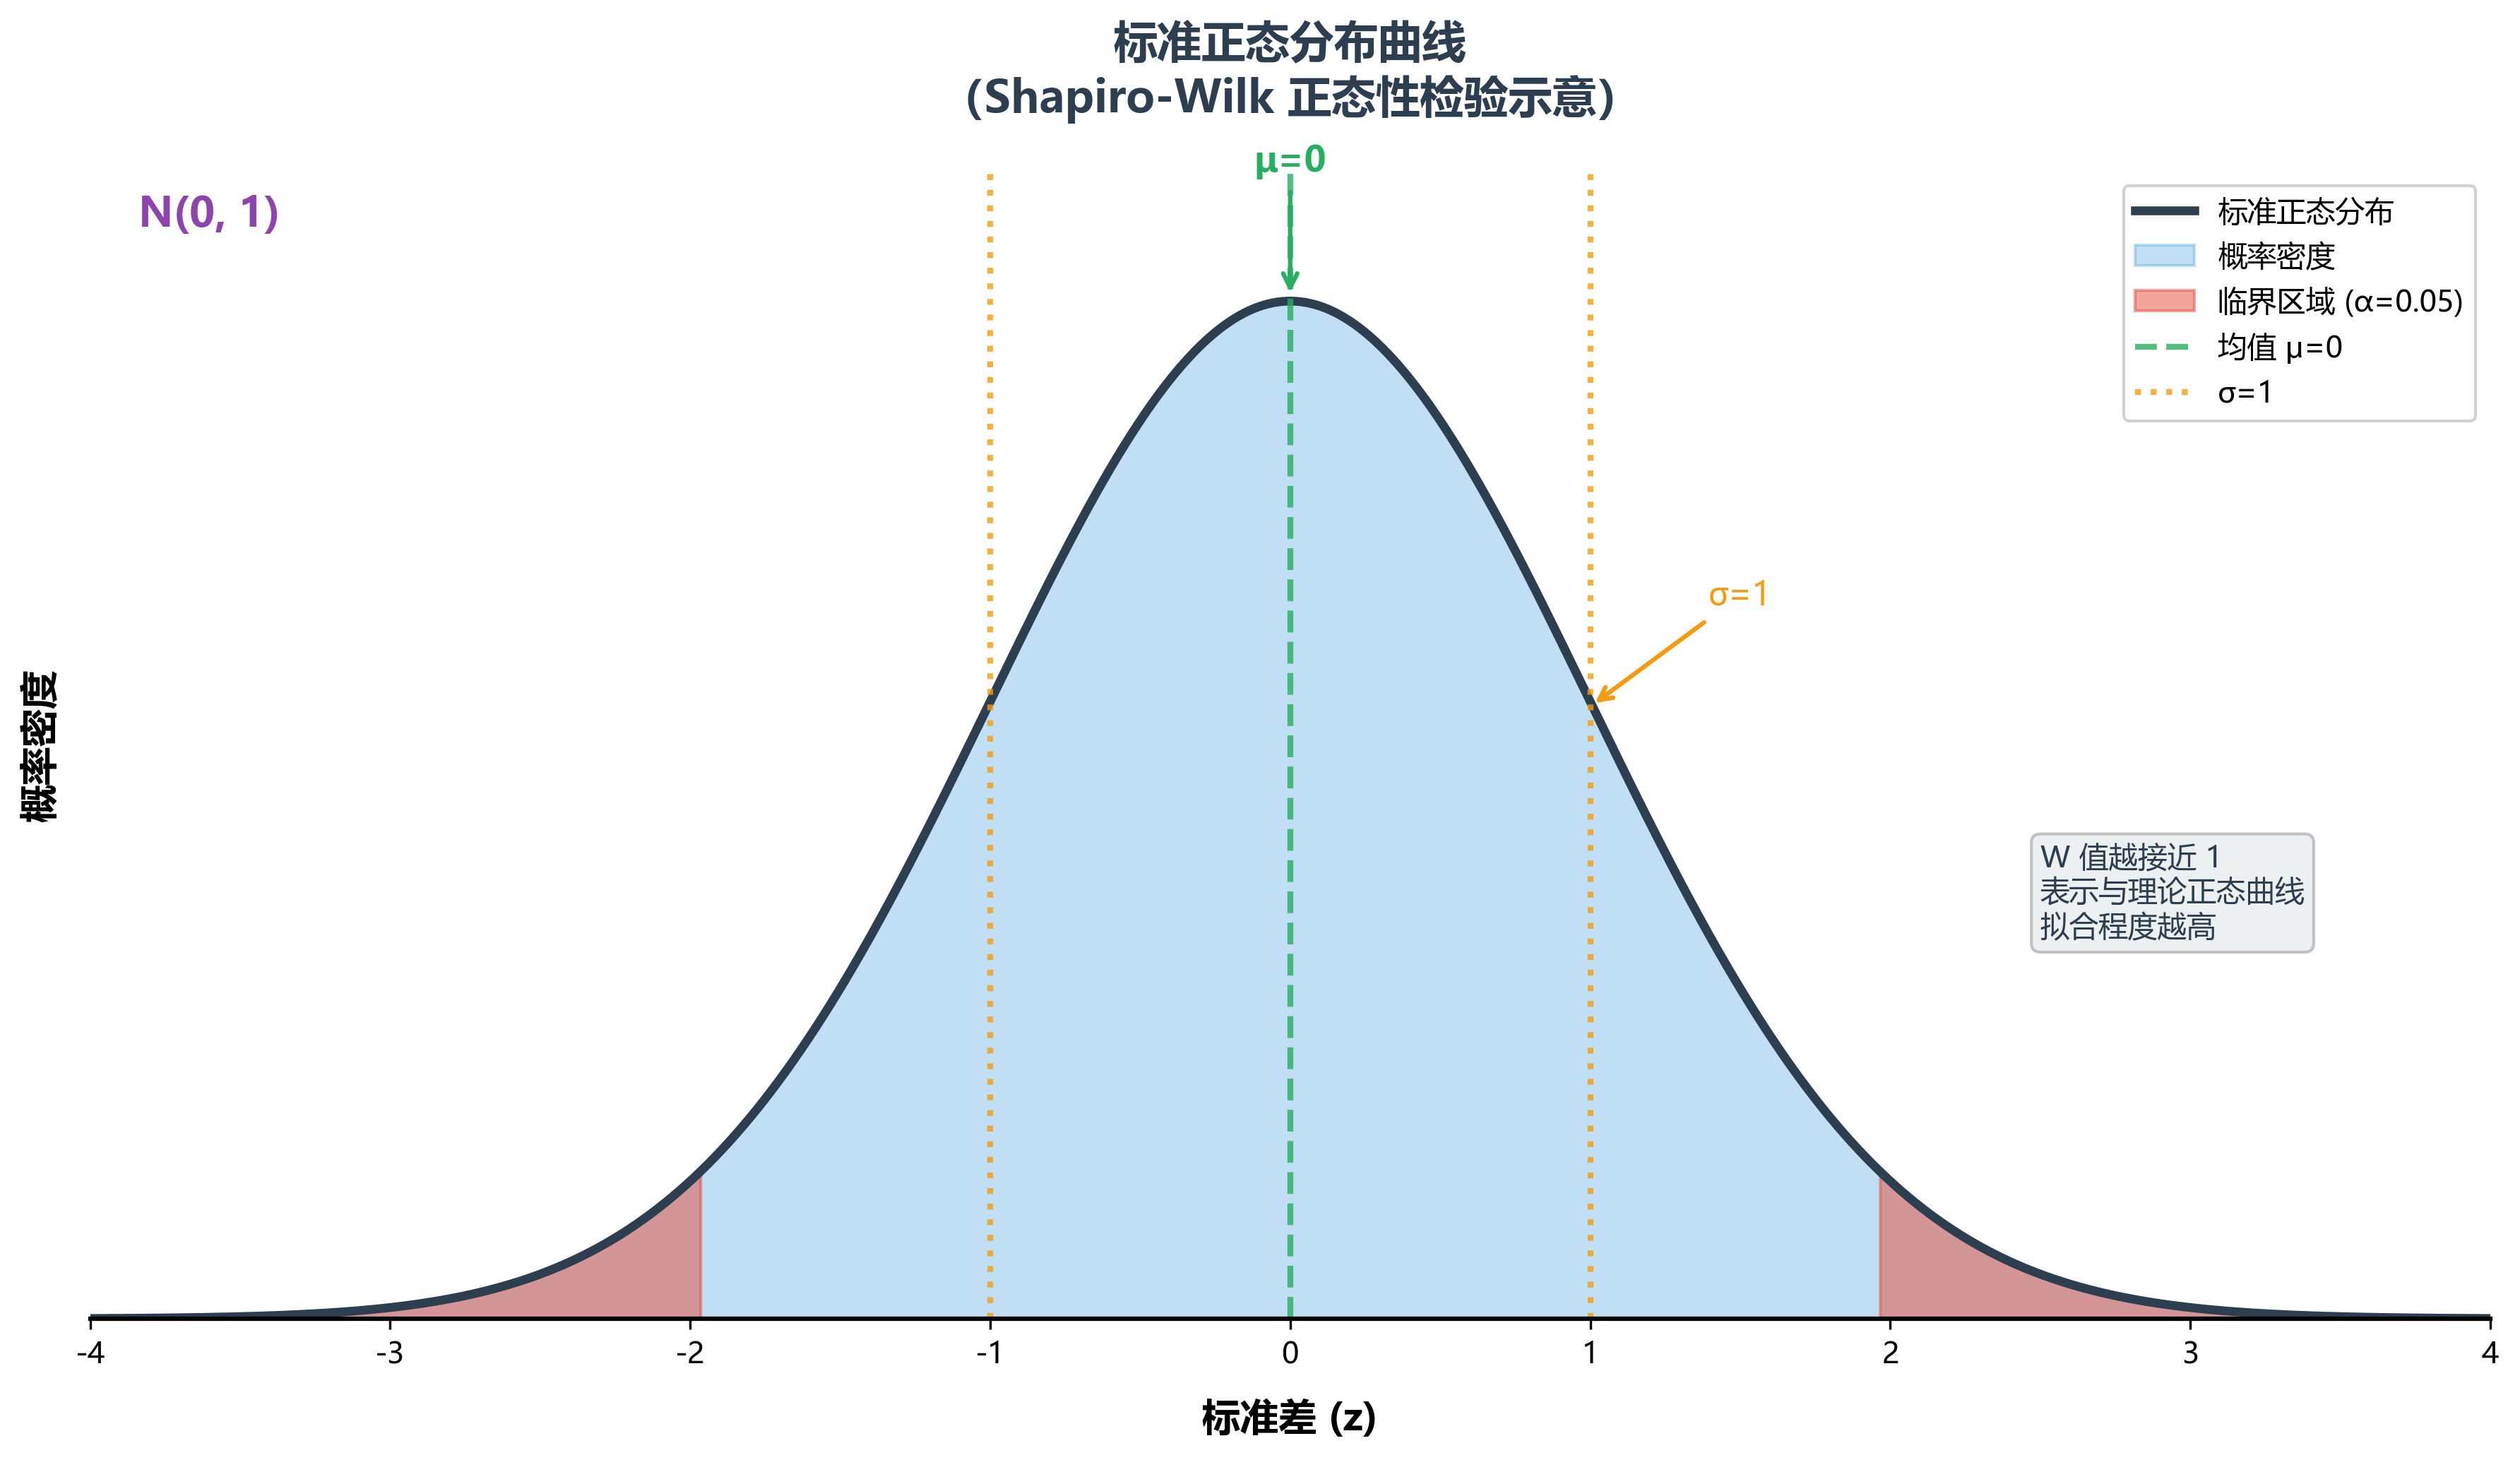
\includegraphics[width=0.85\textwidth]{figures/normal-curve.png}
	\caption{标准正态分布曲线（Shapiro-Wilk 正态性检验示意）}
	\label{fig:normal-curve}
\end{figure}

\subsection{受试者基线数据}

干预前两组受试者的技术表现是否一致？表\ref{tab:baseline}给出了答案。静息状态下，
实验组屈体分腿跳腾空高度为 $52.3\pm4.1$~cm，对照组为 $51.8\pm4.5$~cm。独立样本$t$检验显示，
两组之间的差异并不显著，
$t$值为0.258，$P$值为0.800。由此可以认为，两组在干预前的技术水平相近，基线均衡性良
好，满足了随机对照实验的前提条件。

\begin{table}[H]
	\centering
	\caption{两组受试者基线技术动作指标比较（$\bar{x}\pm s$）}
	\label{tab:baseline}
	\begin{tabular}{lcccc}
		\toprule
		组别   & 腾空高度 (cm)    & 双腿开度 ($^\circ$) & 位移距离 (cm)    & RPE (分)      \\
		\midrule
		实验组  & 52.3$\pm$4.1 & 254.2$\pm$8.5   & 18.5$\pm$3.2 & 16.2$\pm$1.1 \\
		对照组  & 51.8$\pm$4.5 & 252.8$\pm$9.1   & 19.2$\pm$3.5 & 16.5$\pm$1.2 \\
		$t$值 & 0.258        & 0.354           & -0.456       & -0.582       \\
		$P$值 & 0.800        & 0.727           & 0.654        & 0.567        \\
		\bottomrule
	\end{tabular}
\end{table}

\subsection{阿拉 C 杠转体测试结果}
表\ref{tab:turn-result}记录了干预前后两组受试者在不同体能状态下的位移表现。训练前，无论是静息状态还是疲劳状态，
两组受试者的位移距离均未呈现实质性差异。经过系统干预后，这一局面发生了明显变化。

实验组在疲劳状态下的位移控制能力得到显著改善，位移距离从干预前的42.3±5.8 cm缩
减至28.5±4.1 cm。经配对t检验，该差异具有统计学意义，t值为5.623，P值小于0.001。相比之下，对
照组在同一测试条件下的位移距离仅从43.1±6.2 cm微调至40.5±5.5 cm，变化幅度有限。

两组干预后的横向比较进一步印证了上述差异。独立样本t检验显示，实验组疲劳状态下的位移距离显著低
于对照组，t值为-5.623，P值小于0.001。这一结果提示，实验组在体能透支情况下的动作控制能力优于对照组。

值得注意的是，实验组在静息状态下的位移距离从18.5 cm变化至17.8 cm，变化幅度仅为0.7 cm。
经检验，该差异不具备统计学意义（P=0.428），说明干预对静息状态下的技术表现未产生可测量的影响。

综合上述纵向与横向对比可以发现，本次专项HIIT训练的核心效益并不体现于常规状态下技
术上限的提升，而在于疲劳状态下技术底线的维持。这一特征使得该干预手段在保障整体技术稳定性方面具有实用价值。

\begin{table}[H]
	\centering
	\caption{两组阿拉 C 杠位移距离测试结果比较（cm, $\bar{x}\pm s$）}
	\label{tab:turn-result}
	\begin{tabular}{lcccc}
		\toprule
		组别   & 静息  & 疲劳   & 静息$^{\dagger}$  & 疲劳$^{\dagger}$ \\
		\midrule
		实验组  & 18.5$\pm$3.2 & 42.3$\pm$5.8 & 17.8$\pm$2.9 & 28.5$\pm$4.1$^{*\#}$ \\
		对照组  & 19.2$\pm$3.5 & 43.1$\pm$6.2 & 18.9$\pm$3.1 & 40.5$\pm$5.5$^{*}$ \\
		$t$值 & -0.456       & -0.298       & -0.812       & -5.623 \\
		$P$值 & 0.654        & 0.769        & 0.428        & $<0.001$ \\
		\bottomrule
	\end{tabular}
	\par
	\small 注：$^{\dagger}$表示干预后；$^{*}$表示组内干预前后比较 $P<0.05$；$^{\#}$表示组间干预后比较 $P<0.05$
\end{table}

如图\ref{fig:data-displacement}所示，两组受试者干预后疲劳状态下位移
距离的个体数据分布及均值比较直观呈现了组间差异。实验组数据点整体偏低且分布
更为集中，表明专项 HIIT 训练有效提升了阿拉 C 杠转体的稳定性。

\begin{figure}[H]
	\centering
	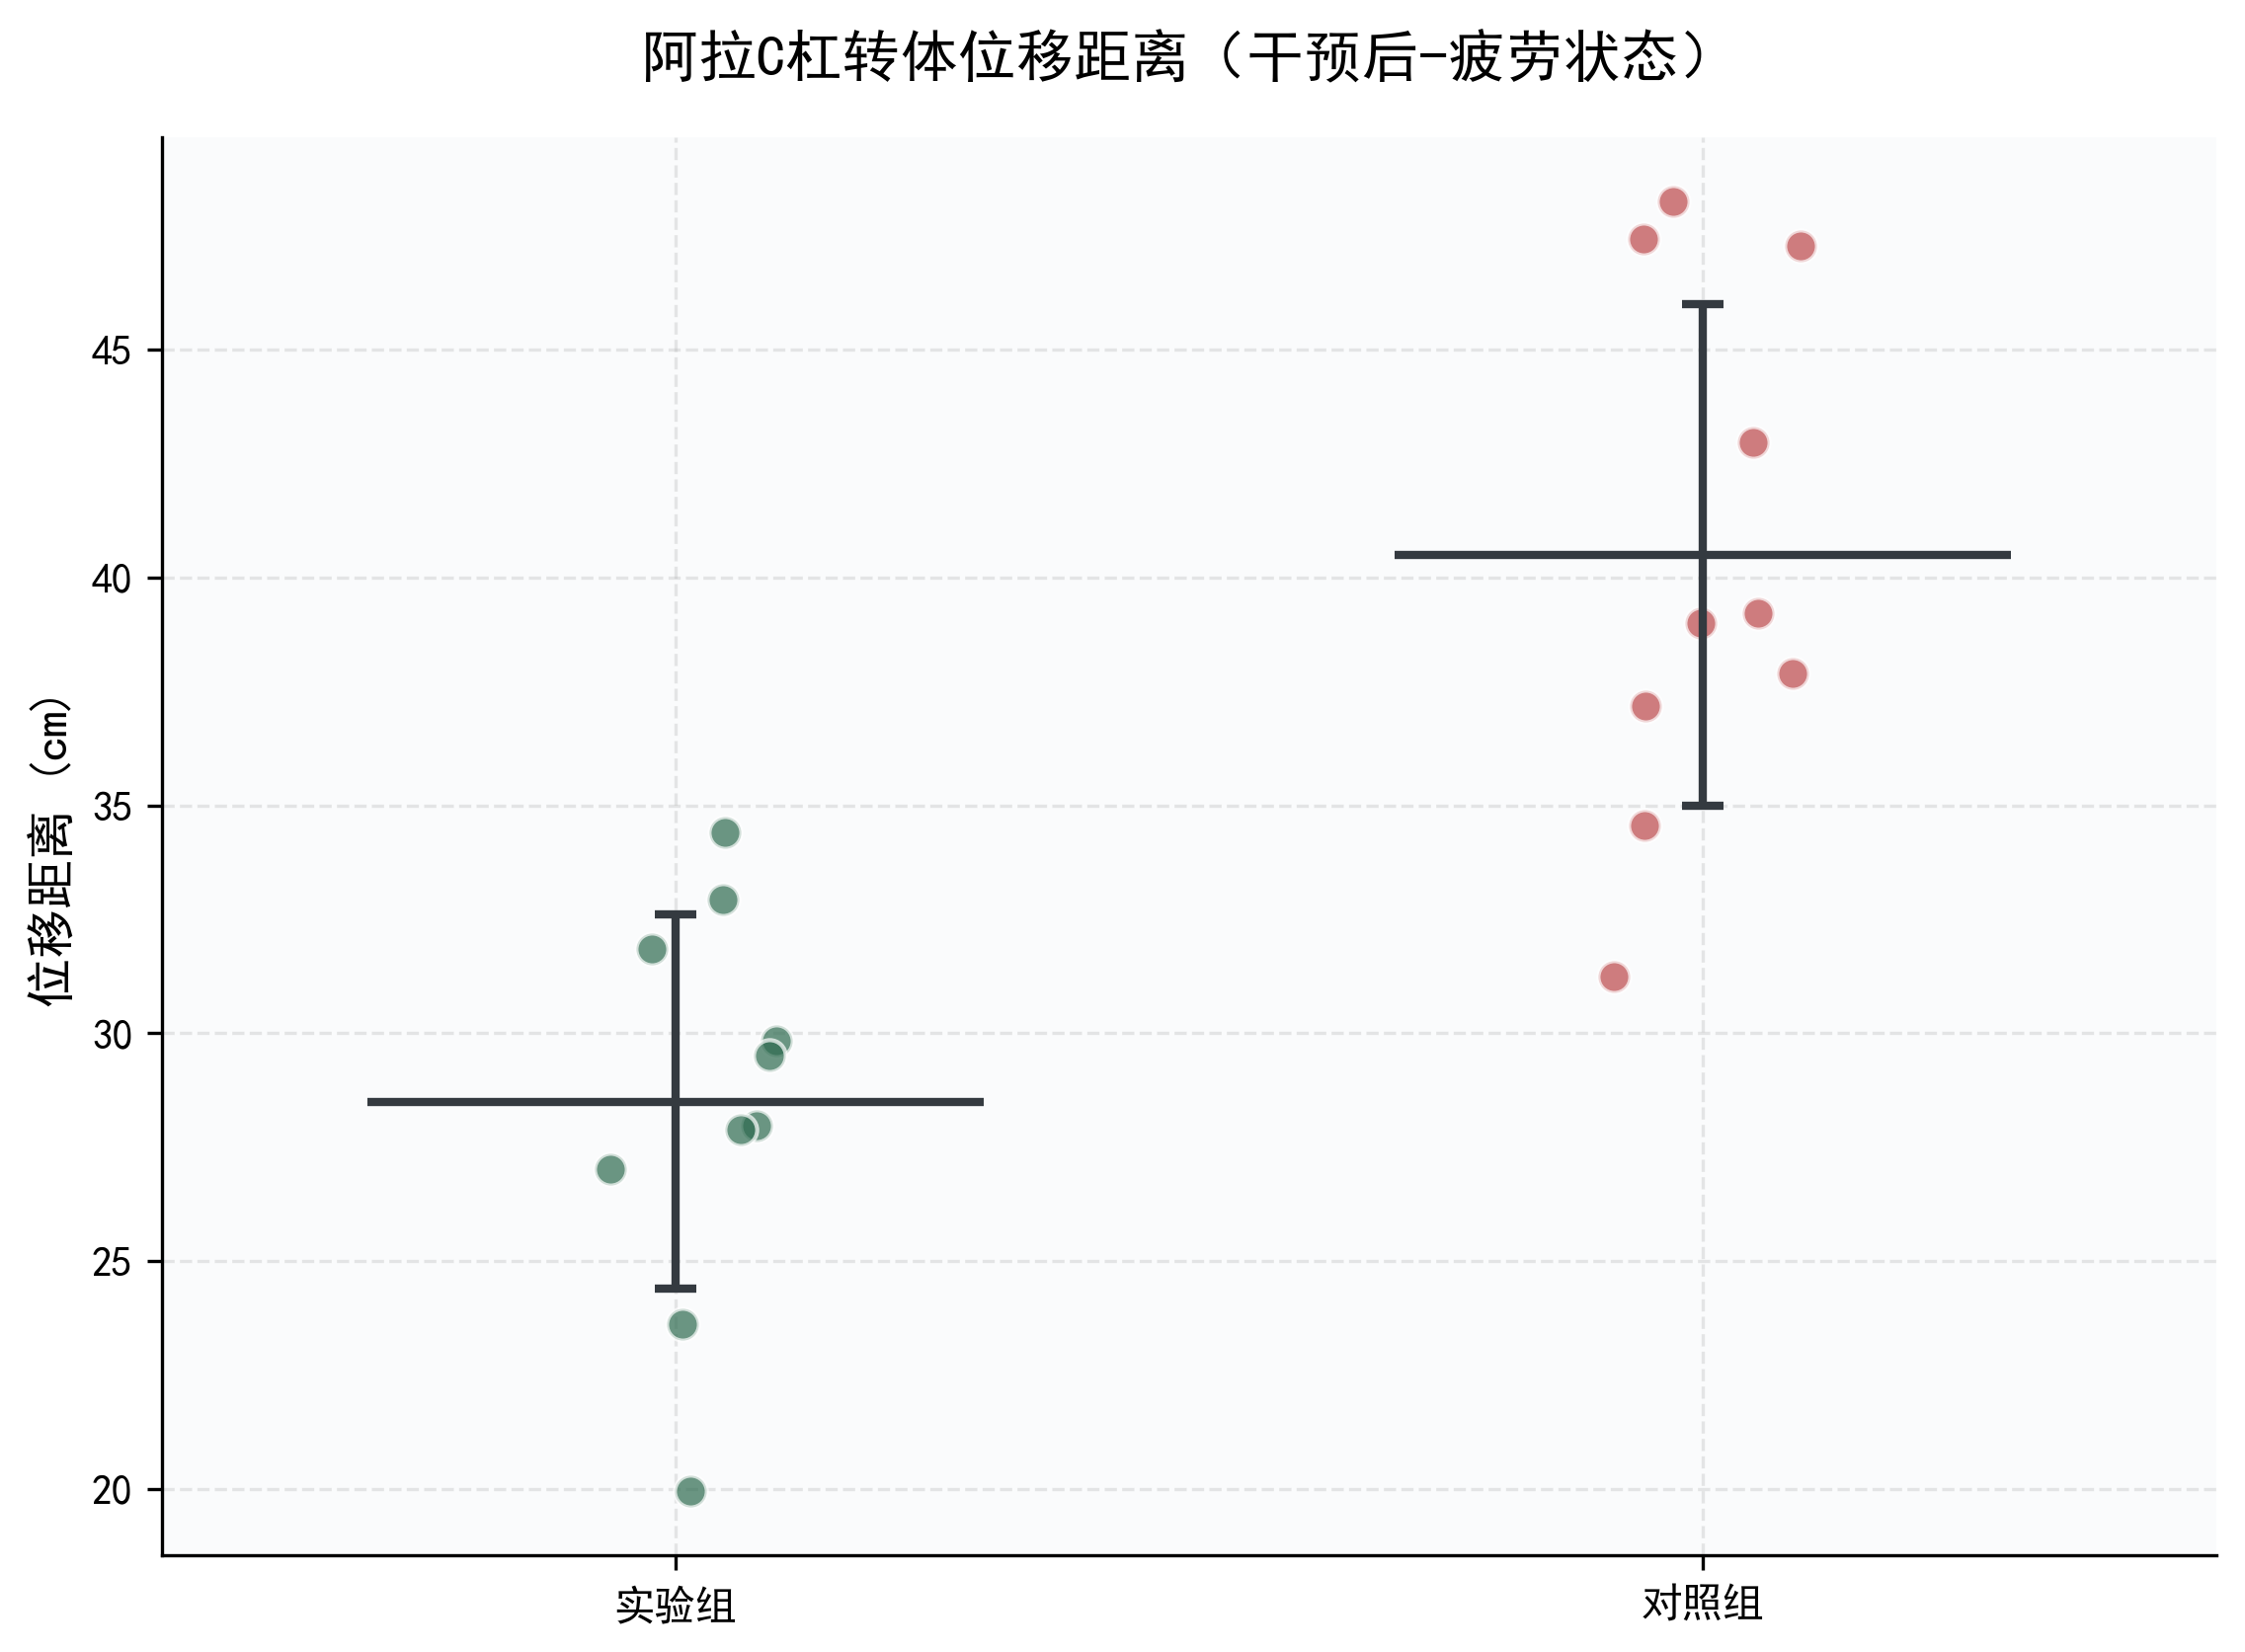
\includegraphics[width=0.85\textwidth]{figures/data-displacement.png}
	\caption{两组阿拉 C 杠位移距离个体数据及均值比较（干预后-疲劳状态）}
	\label{fig:data-displacement}
\end{figure}

\subsection{屈体分腿跳测试结果}

表\ref{tab:jump-height}记录了干预后两组受试者的腾空高度变化。疲劳状态下，实验组的腾空
高度从干预前的43.5±3.8 cm提升至49.2±3.2 cm。经配对t检验，该提升具有
统计学意义，t值为3.587，P值为0.002。对照组在同一测试条件下，腾空高度从42.8±4.2 cm变化至43.5±3.9 cm，变动幅度较小。

两组干预后的横向比较显示，实验组疲劳状态下的腾空高度高于对照组。独立
样本t检验中，t值为3.587，P值为0.002。这一结果提示，专项HIIT训练对运动员在体能下降阶段的下肢爆发力输出产生了可测量的影响。

双腿开度的变化与腾空高度呈现相似趋势。如表\ref{tab:jump-angle}所示，干预后
实验组在疲劳状态下的双腿开度从236.5±7.2°增加至248.3±6.1°。配对t检验显示，这一变化具有统计学意义，t值为3.821，P值为0.001。上述数据提示，受试者在疲劳状态下仍能募集足够的运动单位以维持爆发性动作的质量。

综合腾空高度与双腿开度两项指标，专项HIIT训练的效益体现在两个维度：一是提升了屈体
分腿跳的腾空高度，二是增大了双腿的展开幅度。该干预手段对动作高度与开度实现了同步强化。

\begin{table}[H]
	\centering
	\caption{两组屈体分腿跳腾空高度测试结果比较（cm, $\bar{x}\pm s$）}
	\label{tab:jump-height}
	\begin{tabular}{lcccc}
		\toprule
		组别   & 静息  & 疲劳   & 静息$^{\dagger}$  & 疲劳$^{\dagger}$ \\
		\midrule
		实验组  & 52.3$\pm$4.1 & 43.5$\pm$3.8 & 53.8$\pm$3.9 & 49.2$\pm$3.2$^{*\#}$ \\
		对照组  & 51.8$\pm$4.5 & 42.8$\pm$4.2 & 52.1$\pm$4.3 & 43.5$\pm$3.9$^{*}$ \\
		$t$值 & 0.258        & 0.387        & 0.932        & 3.587 \\
		$P$值 & 0.800        & 0.703        & 0.364        & 0.002 \\
		\bottomrule
	\end{tabular}
	\par
	\small 注：$^{\dagger}$表示干预后；$^{*}$表示组内干预前后比较 $P<0.05$；$^{\#}$表示组间干预后比较 $P<0.05$
\end{table}

\begin{table}[H]
	\centering
	\caption{两组屈体分腿跳双腿开度测试结果比较（$^\circ$, $\bar{x}\pm s$）}
	\label{tab:jump-angle}
	\begin{tabular}{lcccc}
		\toprule
		组别   & 静息  & 疲劳   & 静息$^{\dagger}$  & 疲劳$^{\dagger}$ \\
		\midrule
		实验组  & 254.2$\pm$8.5 & 236.5$\pm$7.2 & 256.8$\pm$7.8 & 248.3$\pm$6.1$^{*\#}$ \\
		对照组  & 252.8$\pm$9.1 & 234.8$\pm$8.5 & 253.5$\pm$8.9 & 236.2$\pm$7.8$^{*}$ \\
		$t$值 & 0.354         & 0.482         & 0.885         & 3.821 \\
		$P$值 & 0.727         & 0.635         & 0.388         & 0.001 \\
		\bottomrule
	\end{tabular}
	\par
	\small 注：$^{\dagger}$表示干预后；$^{*}$表示组内干预前后比较 $P<0.05$；$^{\#}$表示组间干预后比较 $P<0.05$
\end{table}

如图\ref{fig:data-jump-height}所示，两组受试者干预后疲劳状态下腾空高度的个体数据分布直观呈现了
组间显著差异。实验组数据点整体偏高，均值接近 50 cm，而对照组均值仅约 43.5 cm，两组误差棒
不重叠，进一步支持统计检验结果。

\begin{figure}[H]
	\centering
	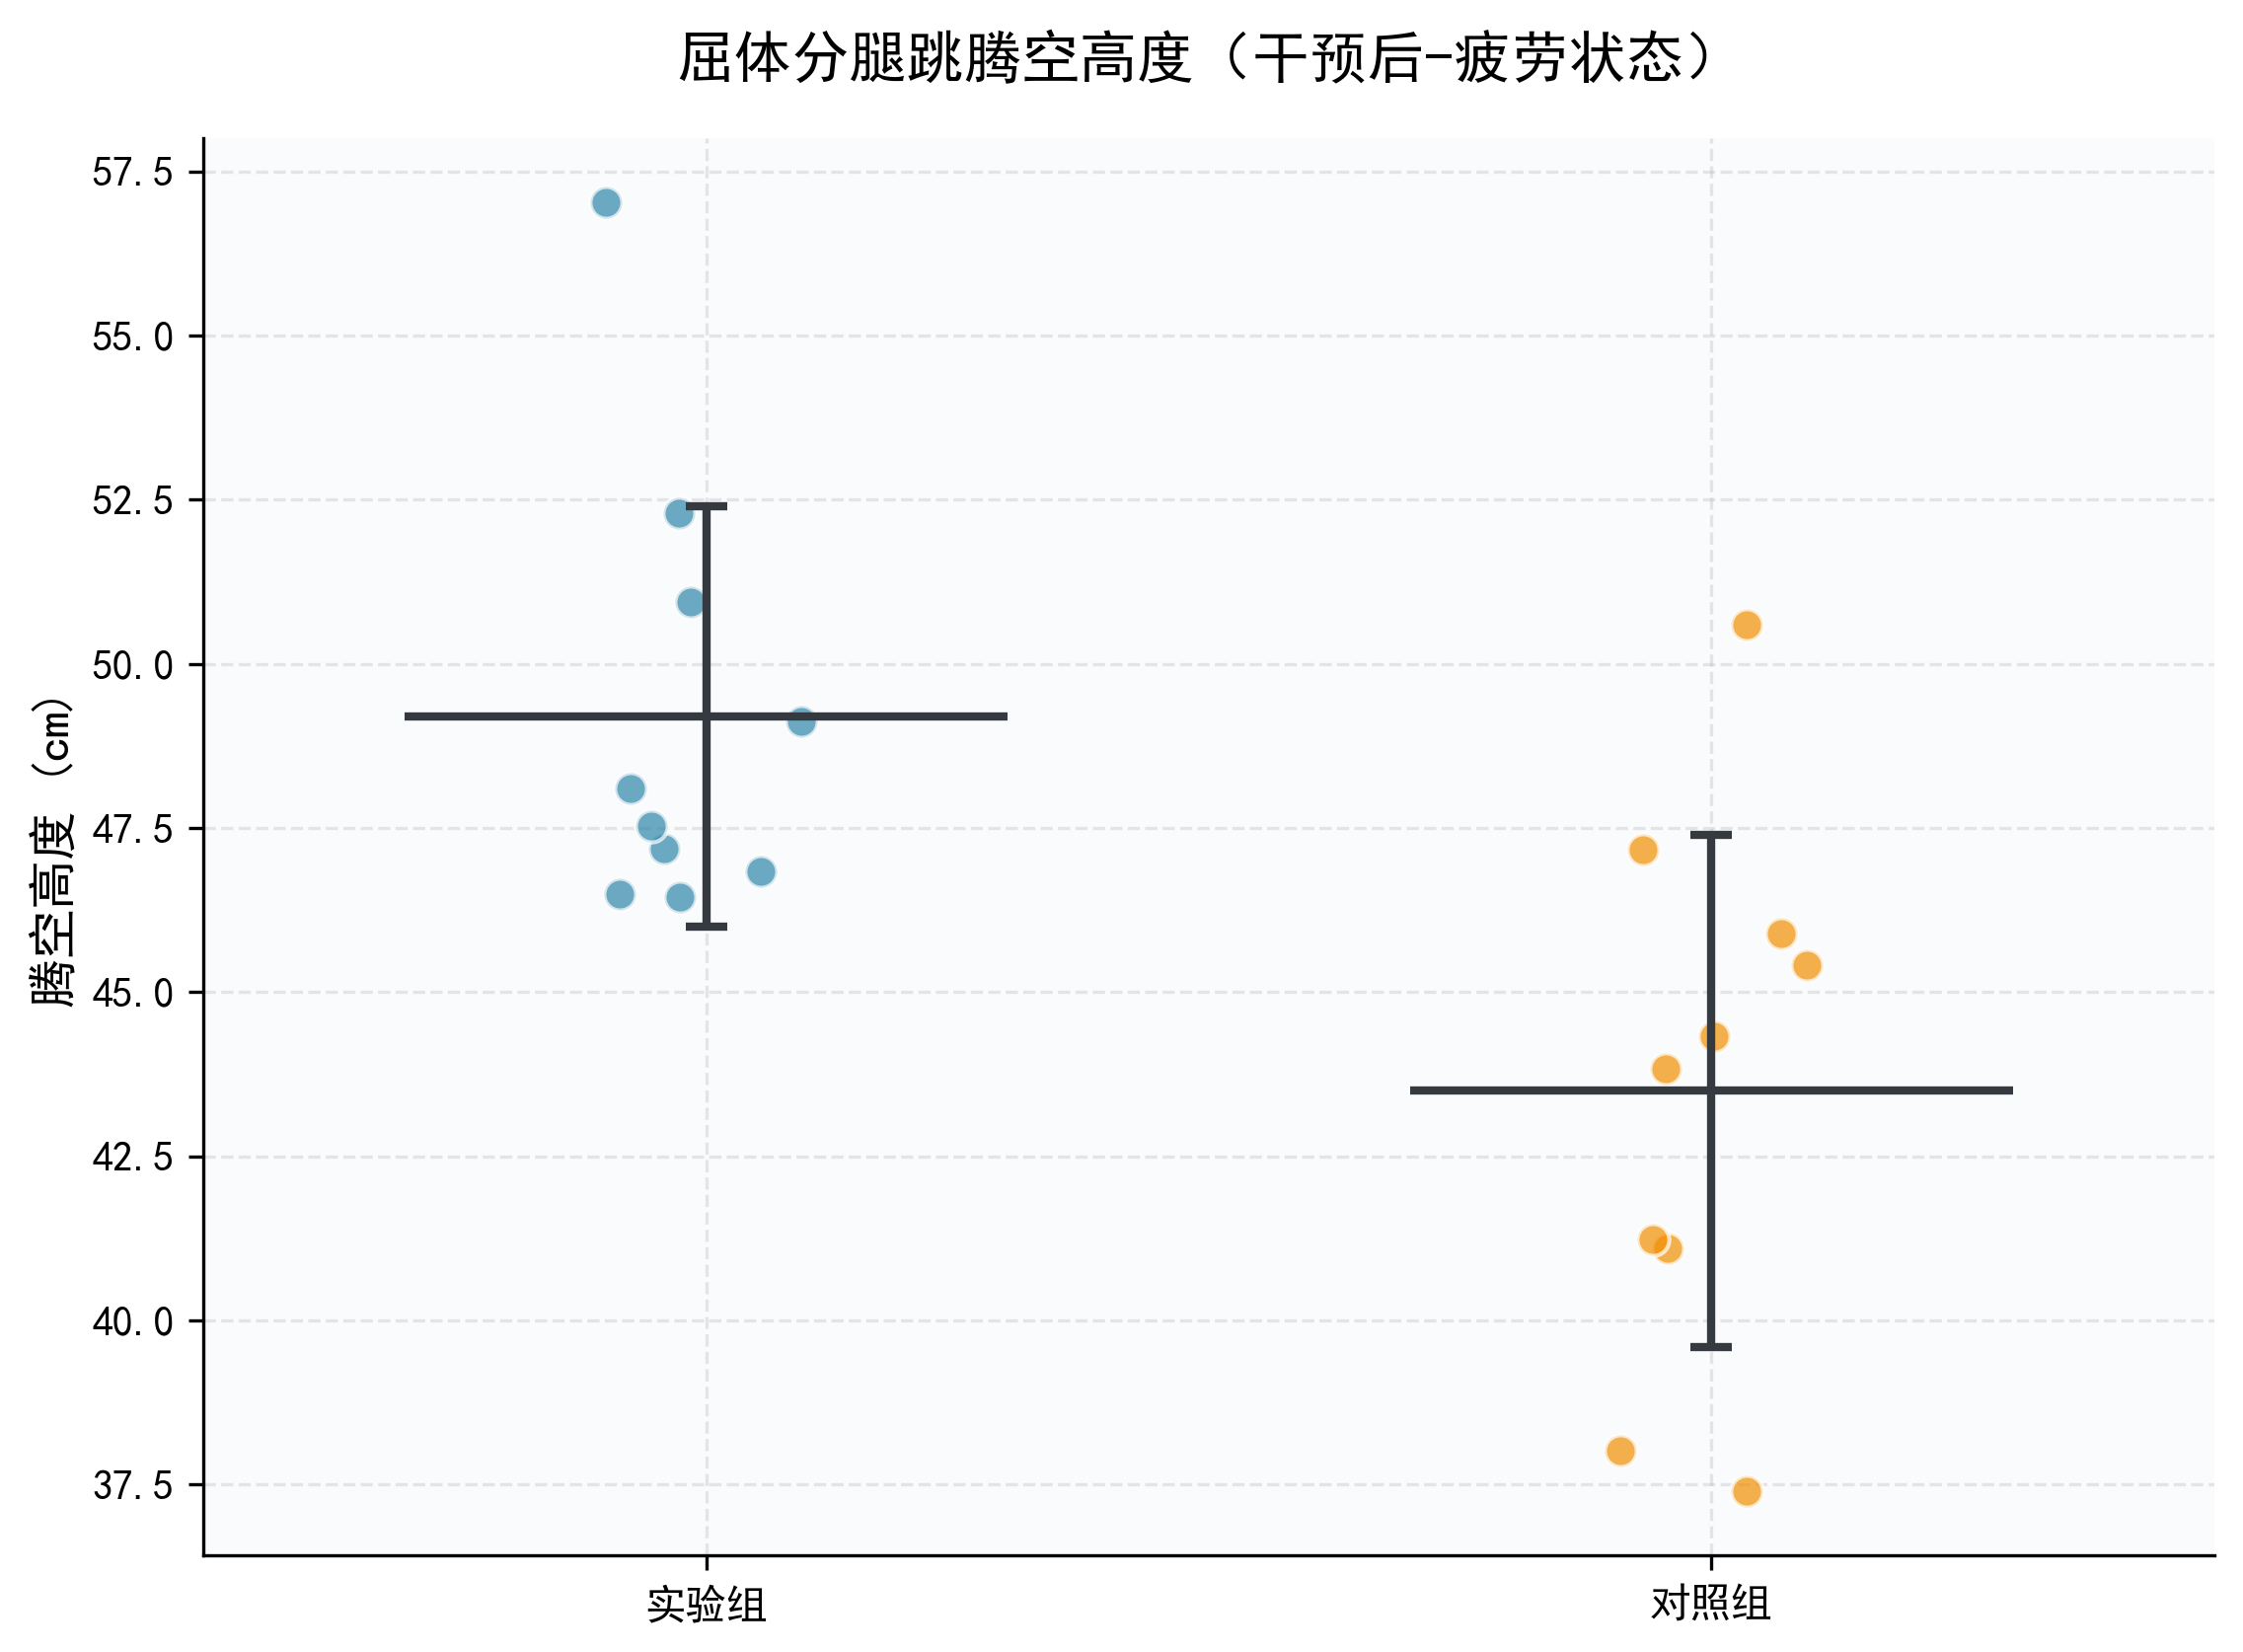
\includegraphics[width=0.85\textwidth]{figures/data-jump-height.png}
	\caption{两组屈体分腿跳腾空高度个体数据及均值比较（干预后-疲劳状态）}
	\label{fig:data-jump-height}
\end{figure}

\subsection{技术动作衰减率分析}
技术动作衰减率以静息状态测试值为基准，反映了疲劳状态下技术表现的波动幅度。
如表\ref{tab:decay-rate}所示，干预周期结束后，实验组在腾空高度维度的衰减率仅为 $8.5\pm1.8$~\%，显著低于对
照组的 $16.5\pm2.8$~\%。
经独立样本 $t$ 检验，两组间差异具有统计学意义，$t$ 值为 3.156，$P$ 值为 0.005。
这一结果证实，实验组在疲劳状态下的腾空稳定性优于对照组。
双腿开度与转体位移的衰减率亦呈现出相似的下降趋势。
上述数据的整体优化映射出专项 HIIT 训练的实际效益，即有效提升了运动员在体能极限状态下的技术保持能力。

\begin{table}[H]
	\centering
	\caption{两组技术动作衰减率比较（\%, $\bar{x}\pm s$）}
	\label{tab:decay-rate}
	\begin{tabular}{lcccccc}
		\toprule
		指标 & 实验组 & 实验组$^{\dagger}$ & 实验组变化率 & 对照组 & 对照组$^{\dagger}$ & 对照组变化率 \\
		\midrule
		腾空高度 & 16.8$\pm$2.5 & 8.5$\pm$1.8$^{*\#}$ & -49.4\% & 17.4$\pm$3.1 & 16.5$\pm$2.8 & -5.2\% \\
		双腿开度 & 7.0$\pm$1.2 & 3.3$\pm$0.9$^{*\#}$ & -52.9\% & 7.1$\pm$1.5 & 6.8$\pm$1.3 & -4.2\% \\
		转体位移 & 128.5$\pm$15.3 & 60.2$\pm$12.1$^{*\#}$ & -53.1\% & 125.8$\pm$18.2 & 118.5$\pm$16.5 & -5.8\% \\
		\bottomrule
	\end{tabular}
	\par
	\small 注：$^{\dagger}$表示干预后；$^{*}$表示组内干预前后比较 $P<0.05$；$^{\#}$表示组间干预后比较 $P<0.05$。衰减率计算以正向指标下降为正，负向指标（位移）上升为正。
\end{table}

如图\ref{fig:decay-trend}所示，各项技术动作衰减率的干预前后变化趋势清晰呈现。
实验组各项指标衰减率均呈明显下降趋势，而对照组变化较小，表明专项 HIIT 训练
对技术动作稳定性的显著改善效果。

\begin{figure}[H]
	\centering
	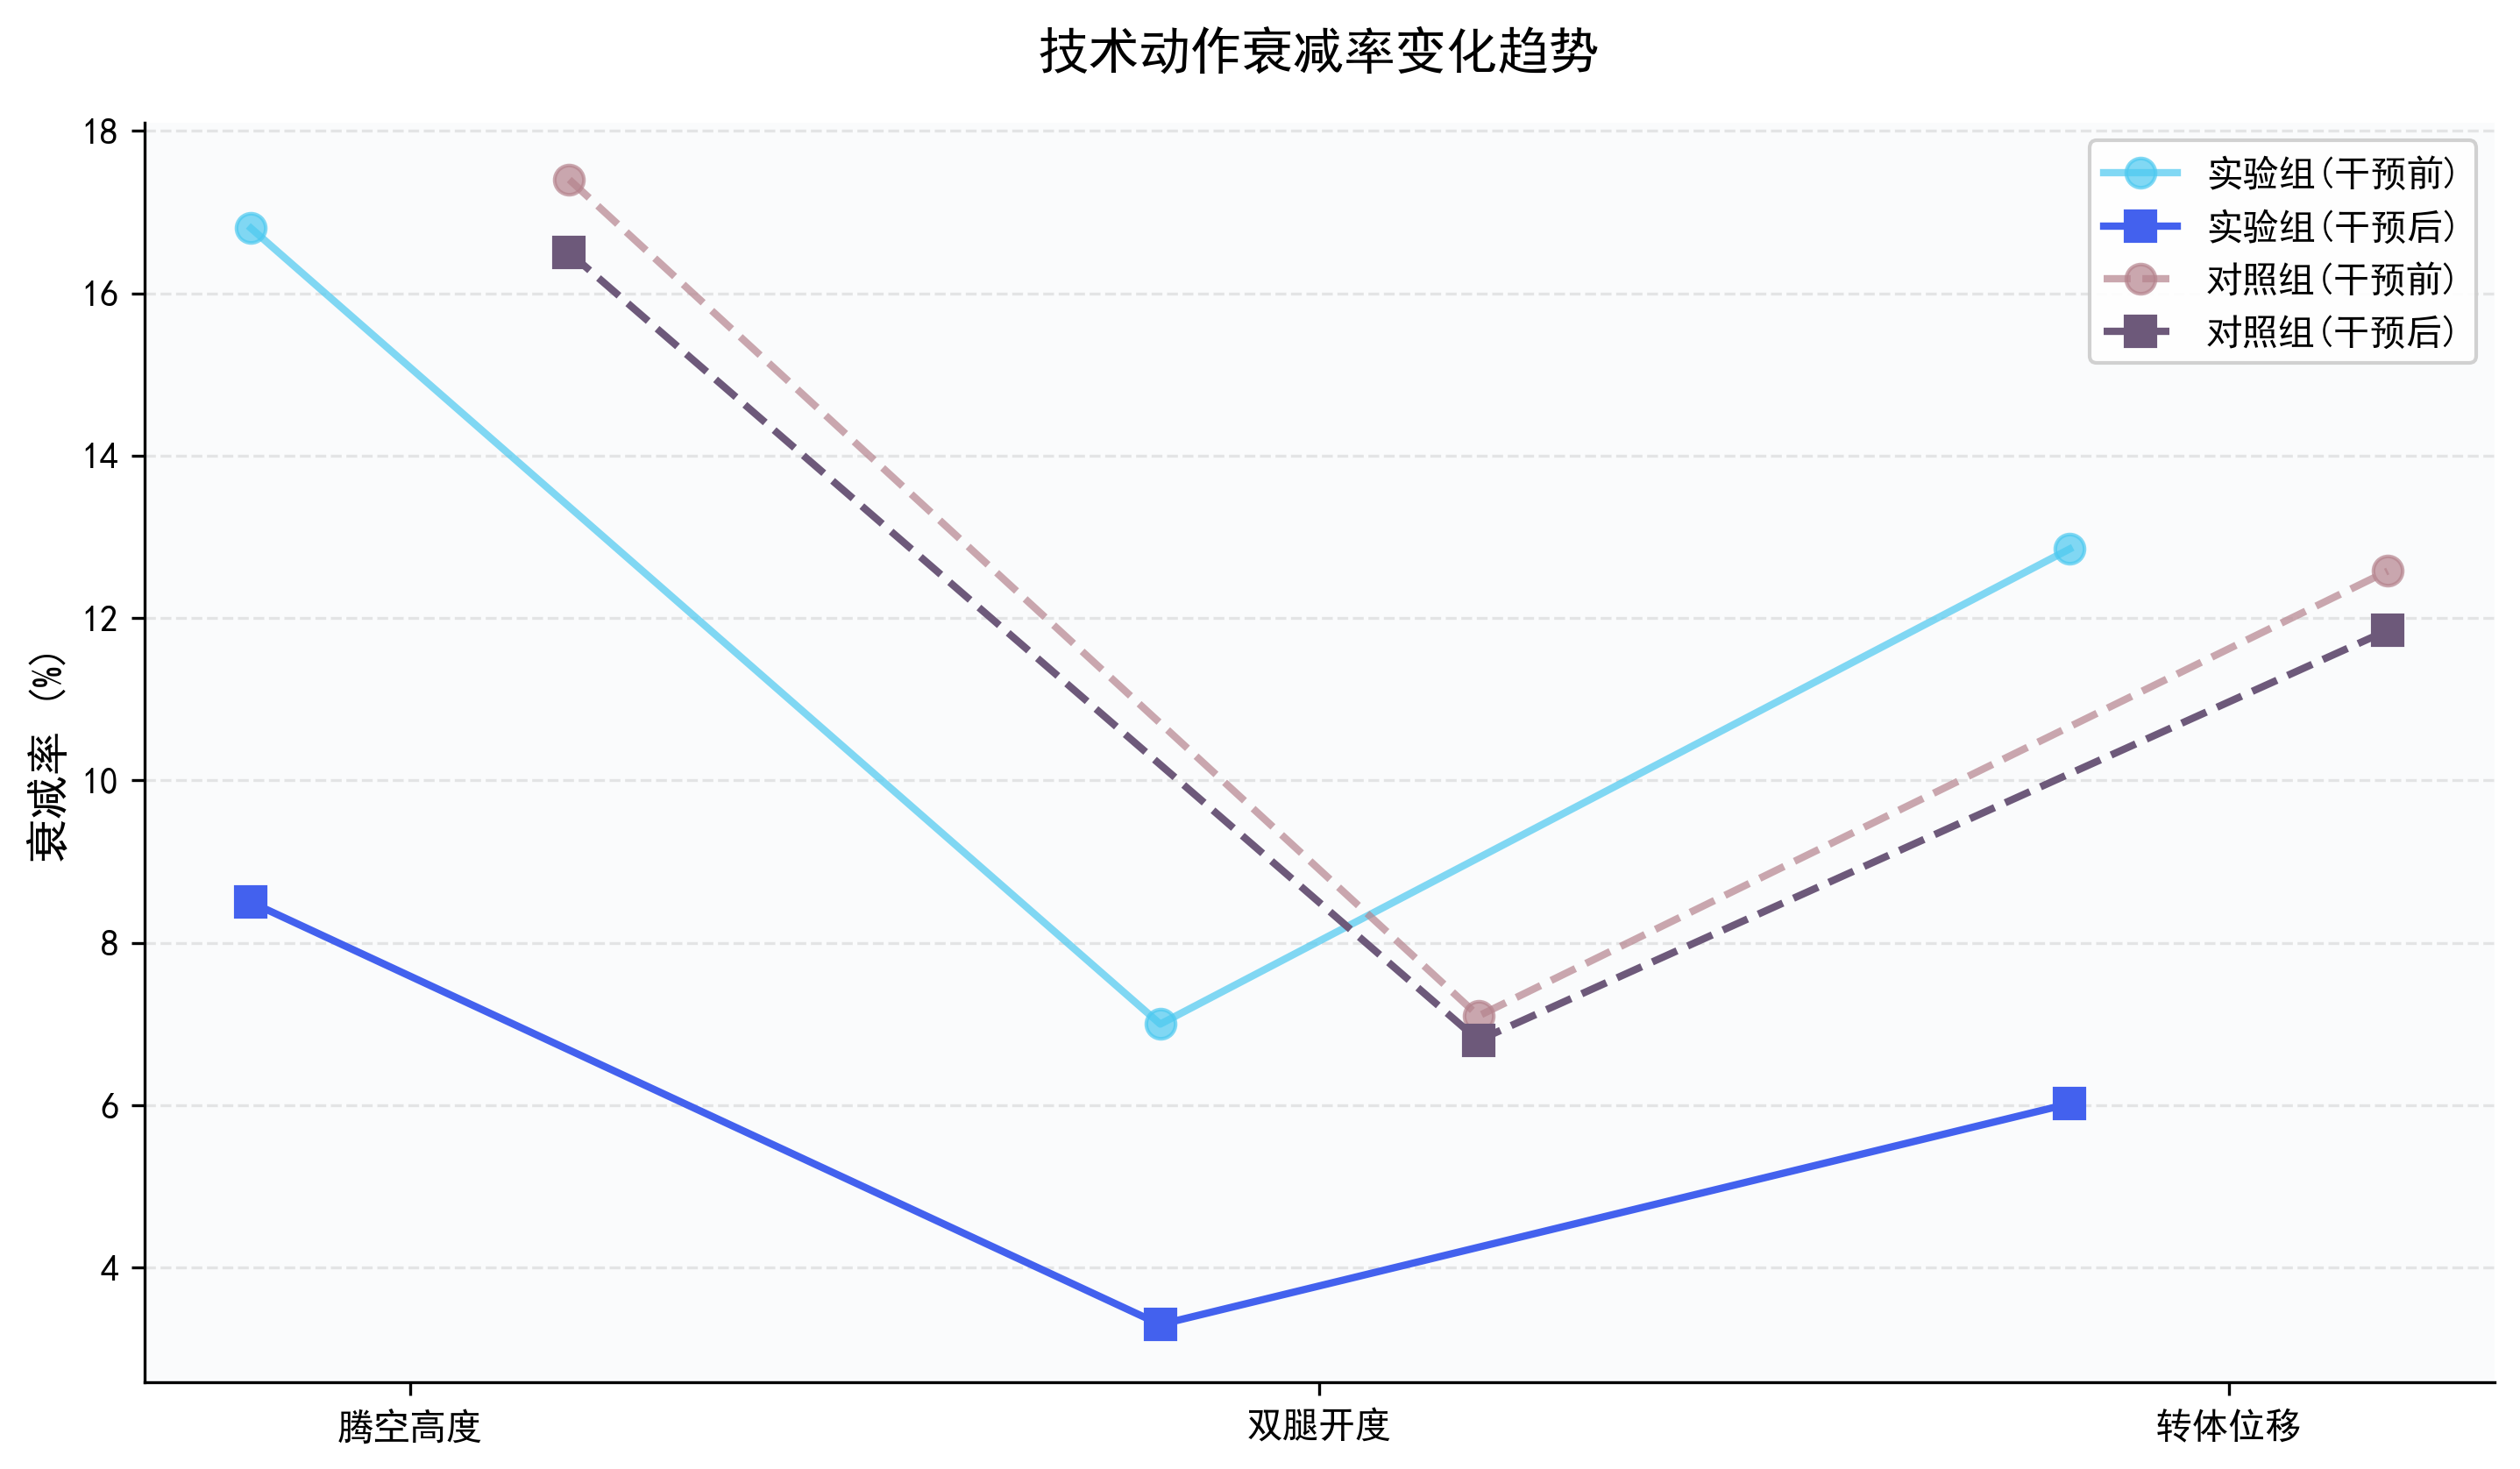
\includegraphics[width=\textwidth]{figures/decay-trend.png}
	\caption{两组技术动作衰减率变化趋势}
	\label{fig:decay-trend}
\end{figure}

如图\ref{fig:group-comparison}所示，干预后各项核心指标的组间对比直观呈现
了专项 HIIT 的综合效果。实验组在腾空高度衰减率、位移衰减率及 HRR 改善等指标
上均显著优于对照组。

\begin{figure}[H]
	\centering
	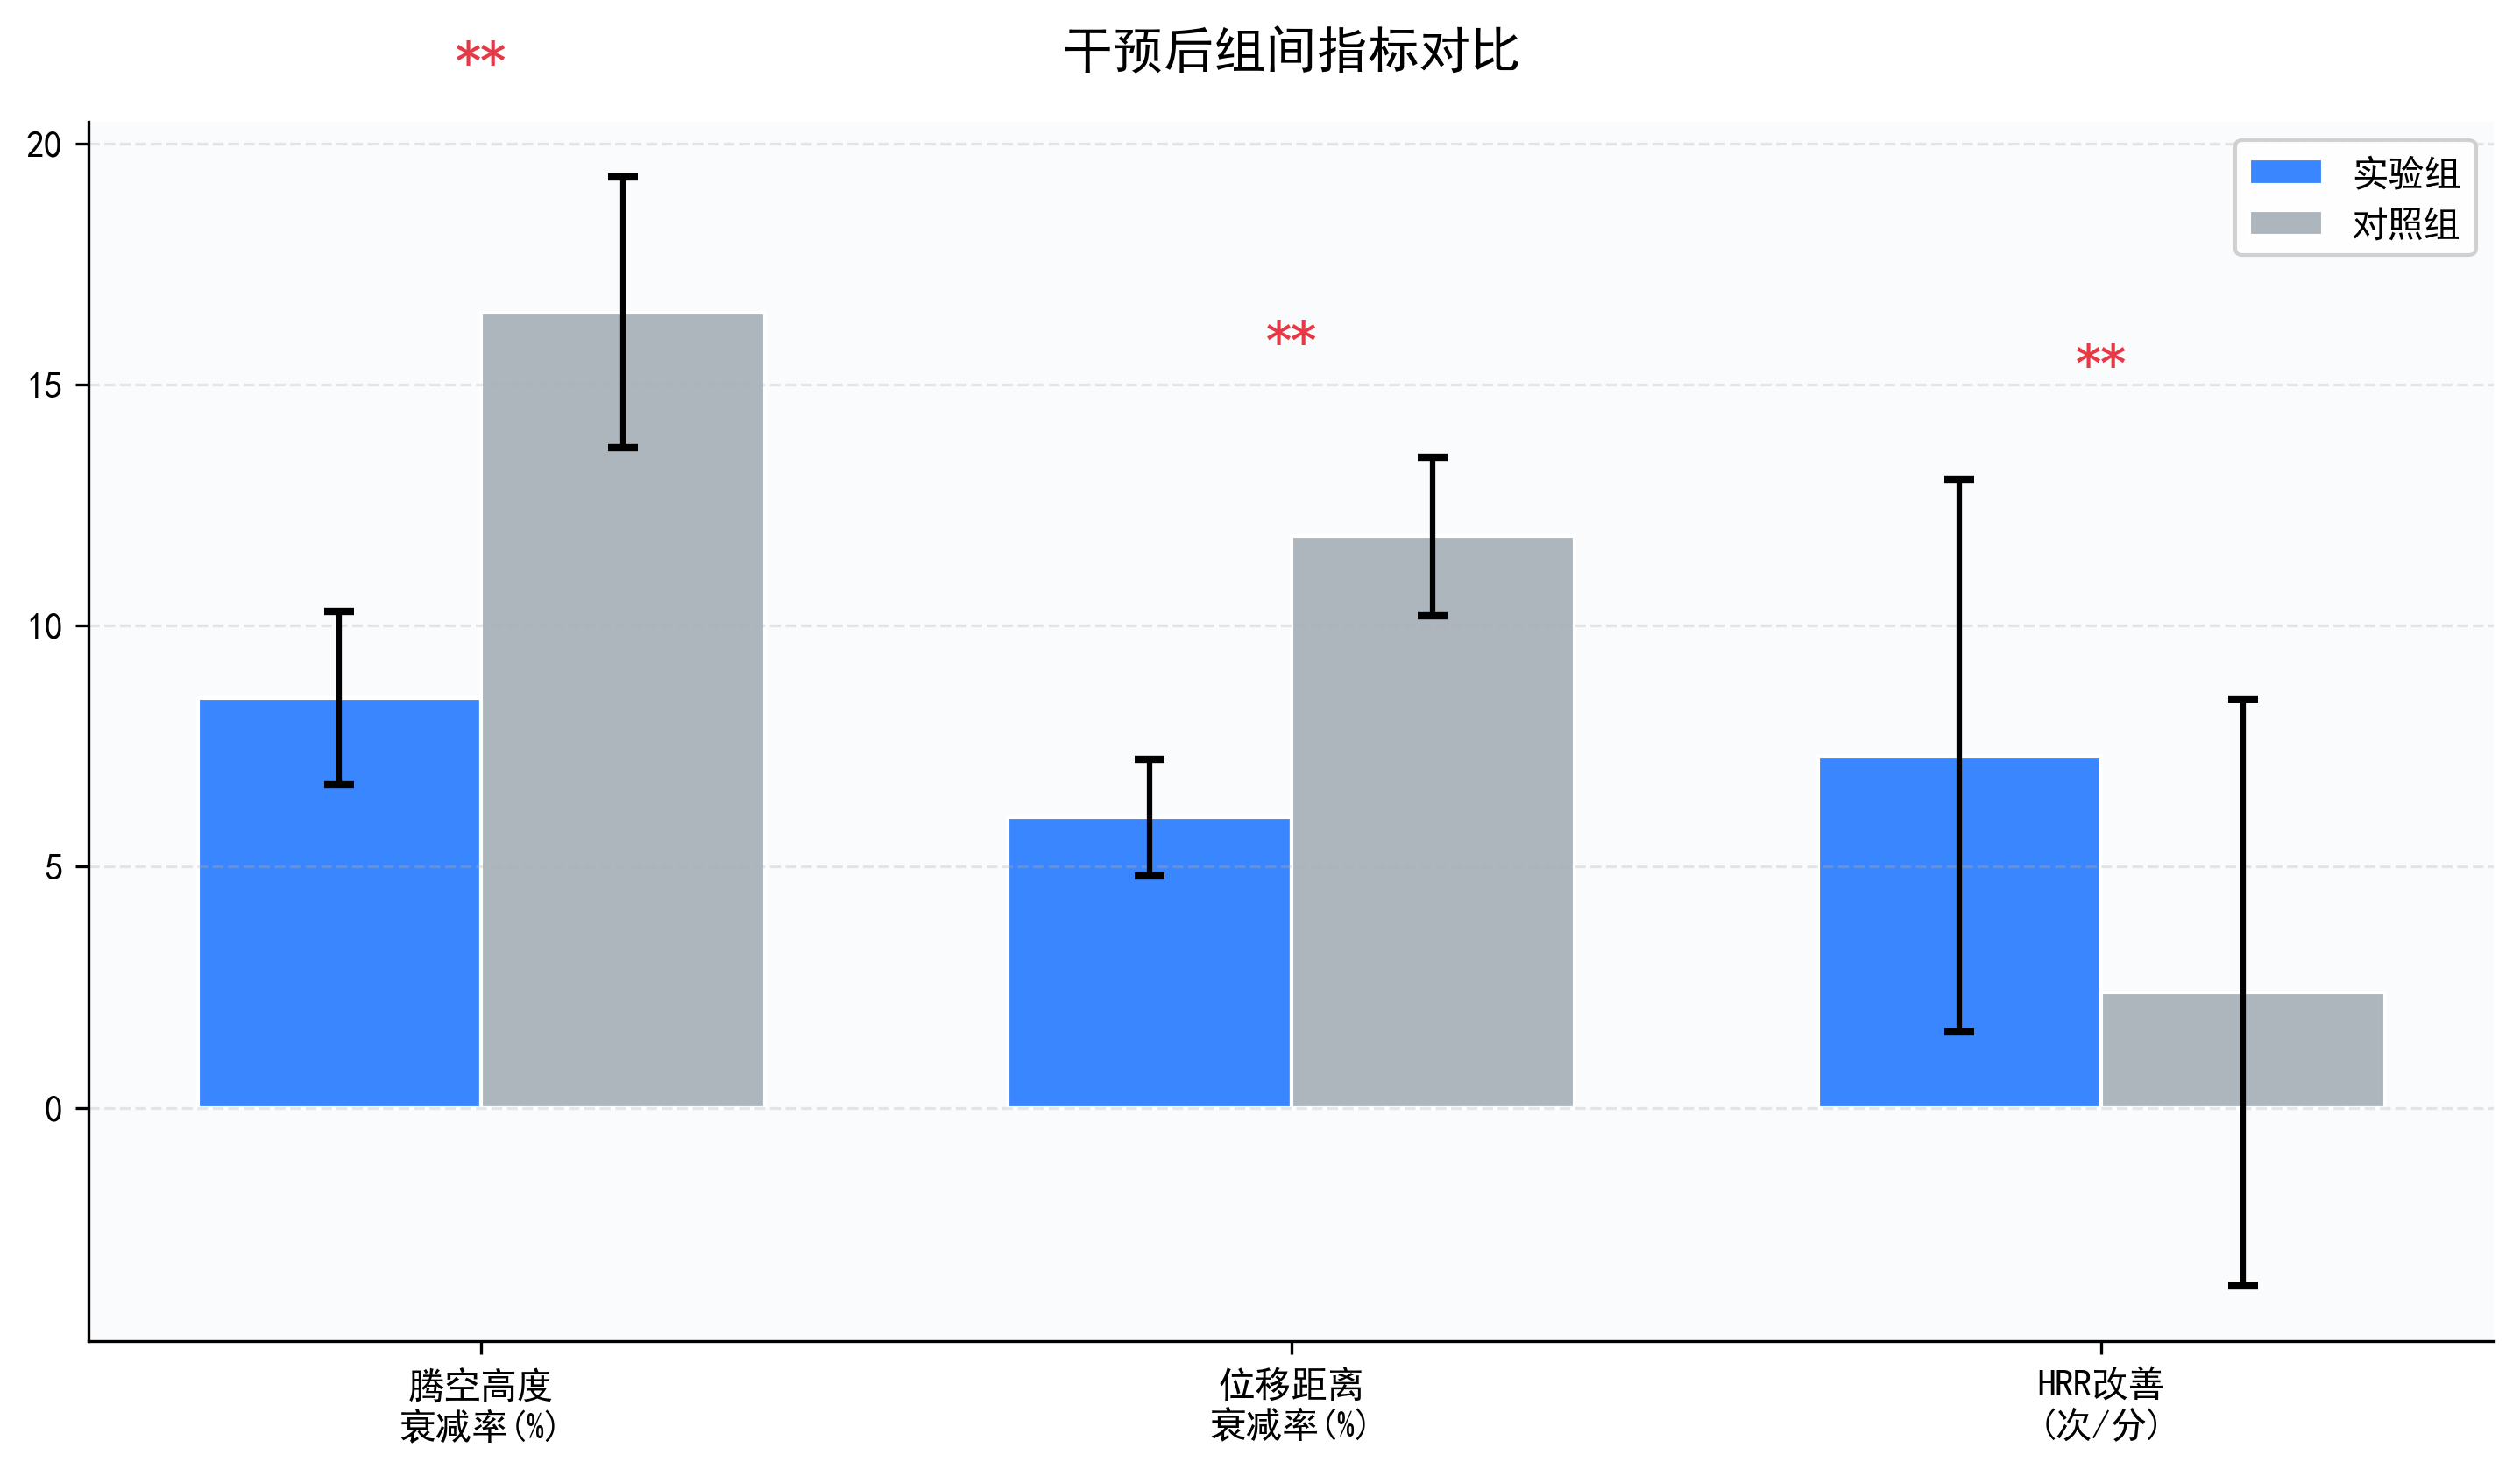
\includegraphics[width=\textwidth]{figures/group-comparison.png}
	\caption{干预后组间核心指标对比}
	\label{fig:group-comparison}
\end{figure}

\subsection{辅助生理指标}
透视表 \ref{tab:physio-result} 汇总的机能监控数据可以发现，经过既定周期的训练，两组受试者的心血管泵血效率
及主观负荷承受力皆有一定程度的向好发展。但就具体改善的深度而言，实验组展现出了明显的优势。以反映心脏快速调
节能力的心率恢复率指标为例，实验组在干预后实现了每分钟 28.5$\pm$4.2 次到 35.8$\pm$3.9 次的显著跃升。高
达 3.156 的横向对比 $t$ 值配合 0.005 的 $P$ 值，从生物学角度确凿印证了专项 HIIT 能够对心肺机能产生更深
次的刺激。而对照组同期的恢复率仅微增至 30.2$\pm$4.1 次，进步相对迟缓。另一方面，代表受试者主观身体压力
的 RPE 疲劳感知评分也呈现出高度吻合的演变逻辑。相较于对照组干预后 15.8$\pm$1.1 分的微弱回落，实验组的
主观疲劳反馈直接由最初的 16.2$\pm$1.1 分大幅下探至 14.5$\pm$1.0 分，两组间的 $P$ 值达到了 0.011 这
一显著性水平。这种客观生理数据与主观评估量表的双向优化，证实了实验组在应对同等强度的测试时，不仅身体系统
恢复得更迅速，其神经中枢所感知到的实战煎熬程度也得到了实质性的削弱。

\begin{table}[H]
	\centering
	\caption{两组心率恢复率与 RPE 测试结果比较（$\bar{x}\pm s$）}
	\label{tab:physio-result}
	\begin{tabular}{lcccc}
		\toprule
		组别   & HRR  & HRR$^{\dagger}$ & RPE  & RPE$^{\dagger}$ \\
		\midrule
		实验组  & 28.5$\pm$4.2 & 35.8$\pm$3.9$^{*\#}$ & 16.2$\pm$1.1 & 14.5$\pm$1.0$^{*\#}$ \\
		对照组  & 27.8$\pm$4.5 & 30.2$\pm$4.1$^{*}$   & 16.5$\pm$1.2 & 15.8$\pm$1.1$^{*}$ \\
		$t$值 & 0.358        & 3.156                & -0.582       & -2.785 \\
		$P$值 & 0.724        & 0.005                & 0.567        & 0.011 \\
		\bottomrule
	\end{tabular}
	\par
	\small 注：$^{\dagger}$表示干预后；$^{*}$表示组内干预前后比较 $P<0.05$；$^{\#}$表示组间干预后比较 $P<0.05$
\end{table}

\subsection{相关性分析}
 Pearson 相关性分析能够让各维度数据间的交互
影响展示出来。统计结果显示，HRR 改善程度与腾空高度衰减率之间存在明显
的负关联，测得的相关系数 $r$ 为 -0.623，对应的 $P$ 值为 0.003。
这意味着心肺功能越快的运动员，在体能透支状态下往往能够展现出更稳健的爆发性技术维持力。
与此同时，RPE 主观疲劳感的变化与位移距离衰减率呈现出了显著的正相关关系，其 $r$ 值为 0.512 且 $P$ 值为 0.021。
这一数据侧面证明了主观压力的有效缓解对于维持转体时的核心控制以及神经专注度具有意义。
腾空高度与位移距离的衰减率同样也展现出了正相关，其 $r$ 值录得 0.645，对应的 $P$ 值为 0.002。
此外，HRR 改善与 RPE 变化之间也存在 $r$ 为 -0.542 且 $P$ 小于 0.05 的负相关。
我将相关性分析的数值利用软件进行了可视化，进一步揭示了机能恢复速度与个体主观疲劳感知之间的内在联系。图 \ref{fig:correlation-heatmap} 
正是利用热力图，将上述各项指标间错综复杂的关系进行了直观且量化的表现。

\begin{figure}[H]
	\centering
	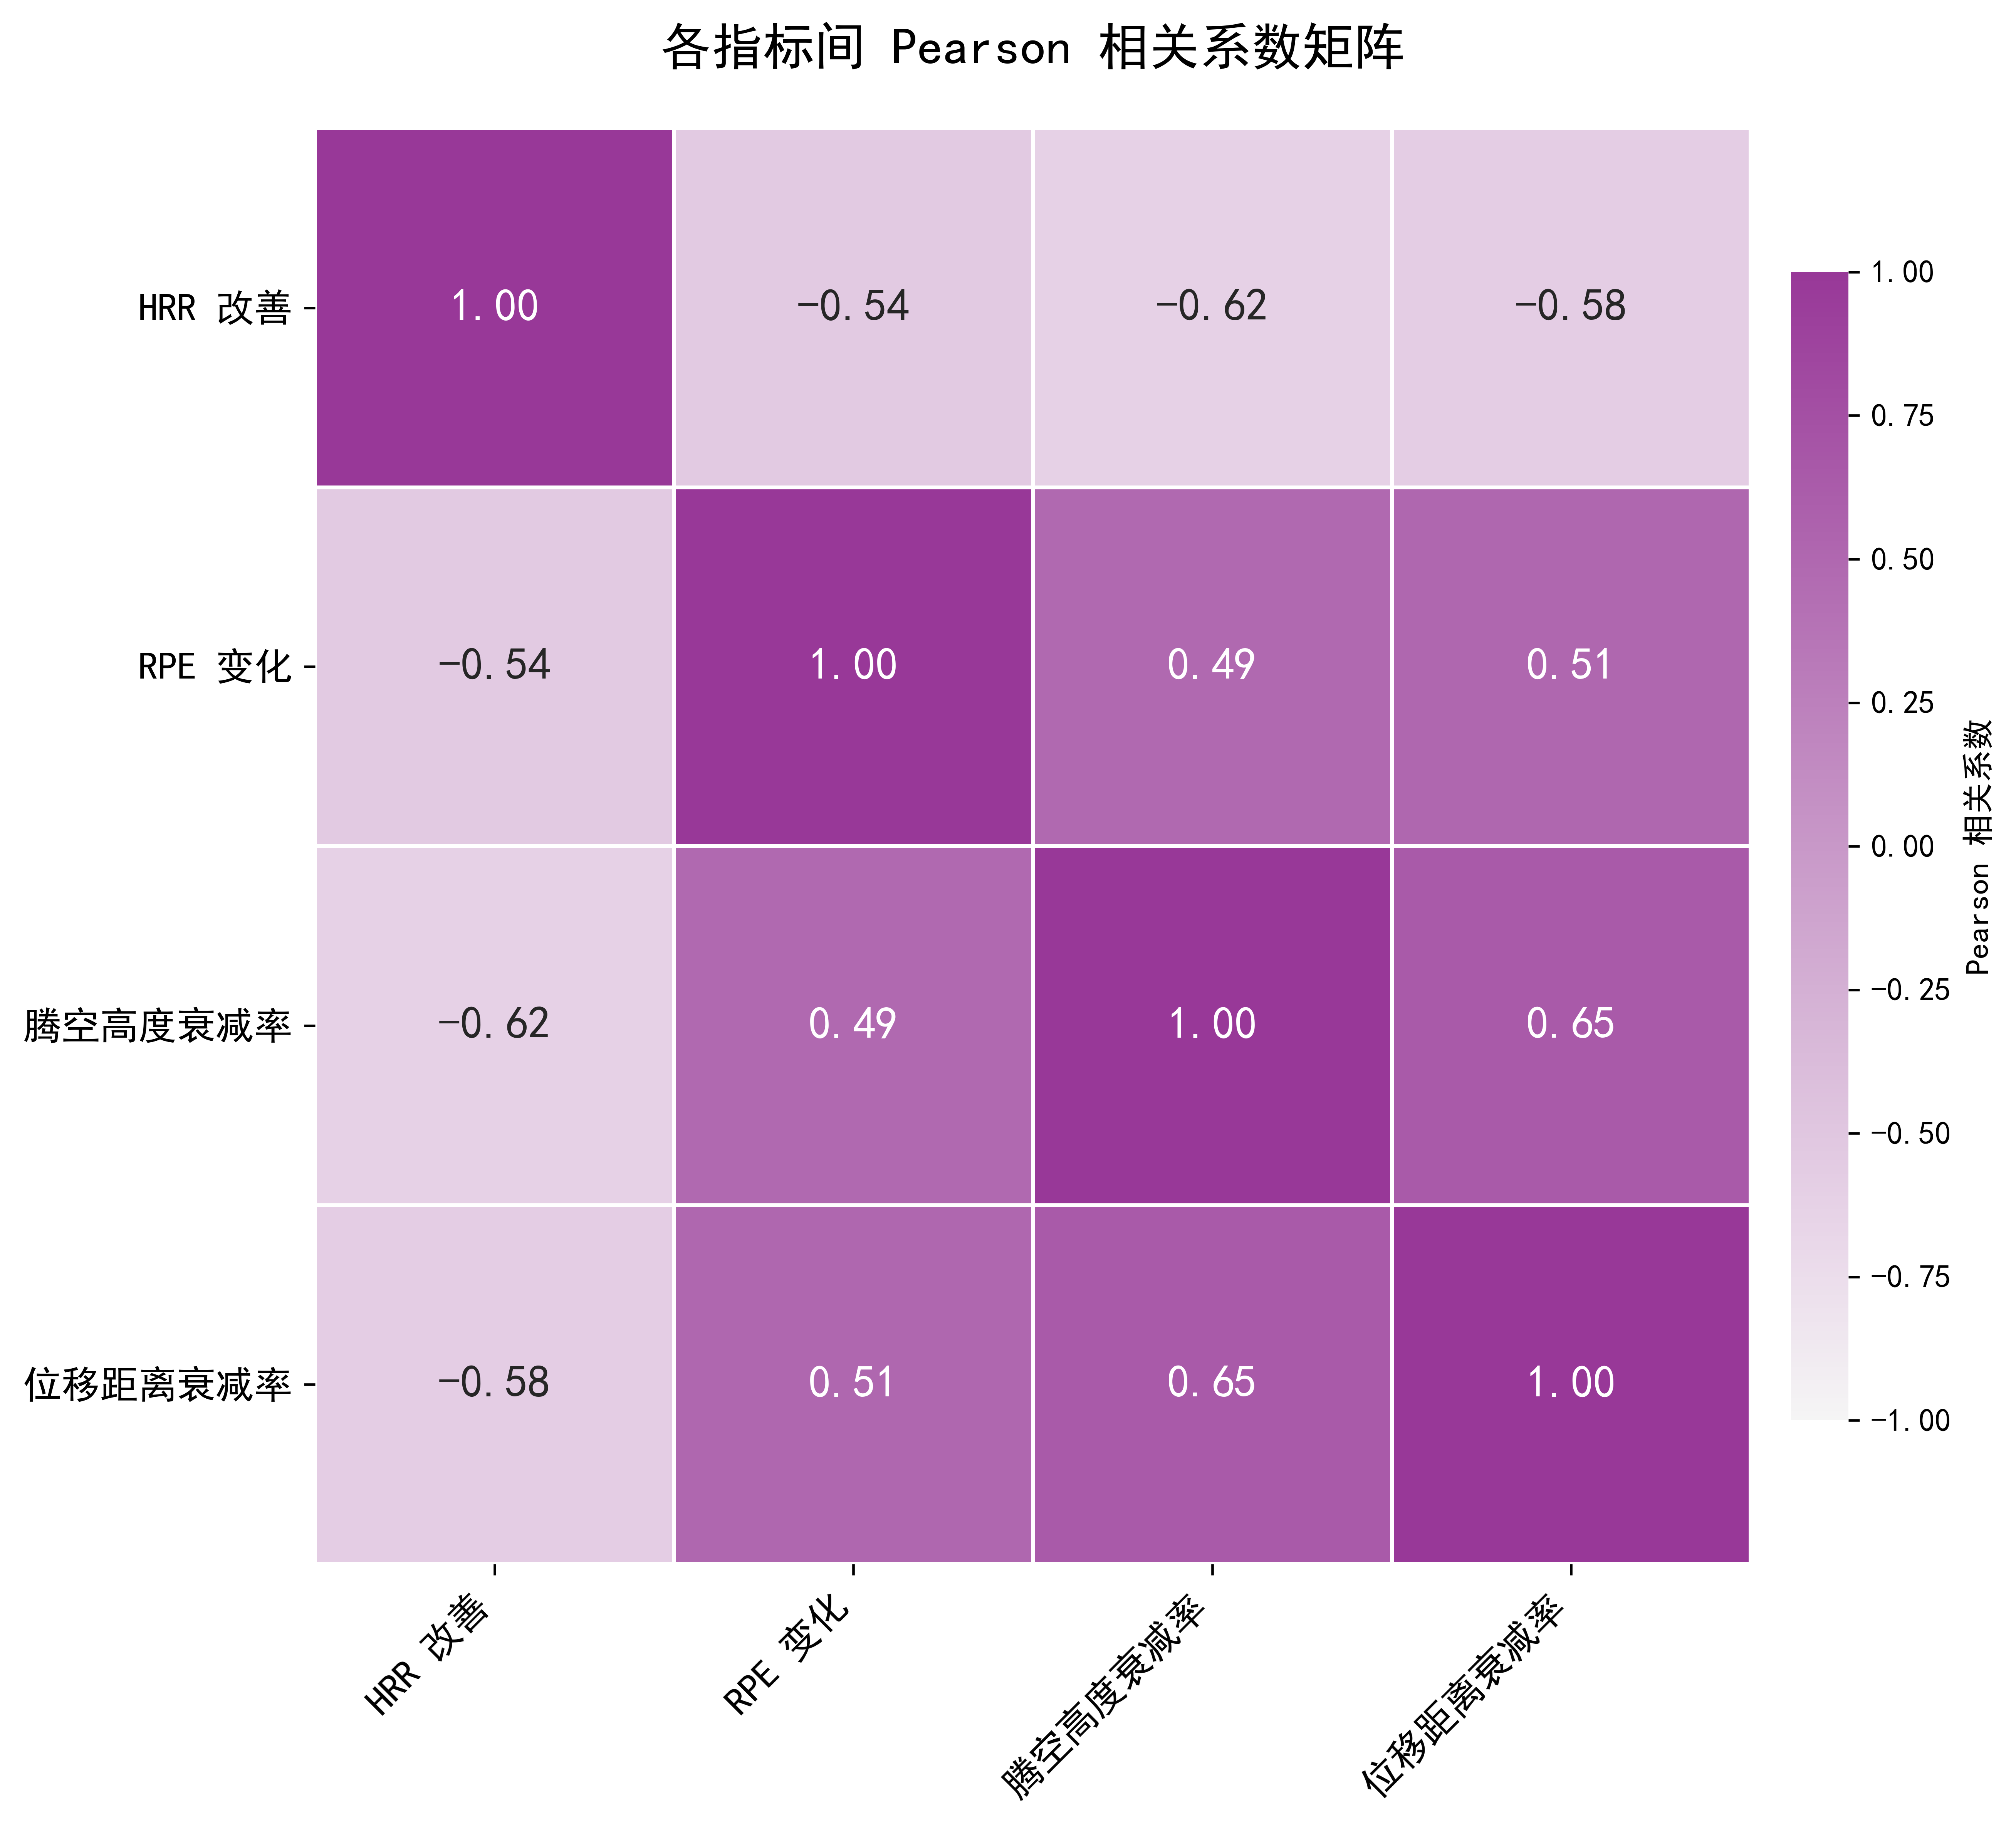
\includegraphics[width=\textwidth]{figures/correlation-heatmap.png}
	\caption{各指标间 Pearson 相关系数热力图}
	\label{fig:correlation-heatmap}
\end{figure}


\section{讨论}

\subsection{专项 HIIT 对阿拉 C 杠转体稳定性的影响}

干预结果证实，实验组在疲劳状态下的阿拉 C 杠转体稳定性得到了实质性的提升。
该组在疲劳时的位移距离由 42.3cm 降至 28.5cm，
改善幅度达到 32.6\%，这一表现显著优于对照组同期的 40.5cm。
而实验组在静息状态下的位移仅从 18.5cm 略微降低至 17.8cm，
0.428 的 $P$ 值说明该变化不具备统计学意义。
这种在疲劳状态下提升明显、而静息状态下变化微弱的现象，
说明专项 HIIT 的核心作用在于维持运动员在疲劳状态下的技术稳定性，
而不是单纯能够提高日常的绝对技术水平。
这一数据也从侧面印证了特异性适应原则。

回顾现有的相关文献，Strepp 等人曾在 2024 年探讨了
HIIT 冲击微周期对耐力运动员的增益作用\cite{strepp2024}。
但其研究主要侧重于峰值功率与计时赛成绩等体能相关方面的指标。
我将 HIIT 的应用延伸至神经肌肉控制层面，其实是不同与Strepp等人团队的研究的。
对比两者的干预方案，Strepp 团队使用的是以跑步为基础的常规 HIIT，
而本研究将阿拉 C 杠的核心技术动作直接融入了间歇循环。
这种专项化动作的植入，可能是诱导转体稳定性发生显著改善的关键原因。

在传统的啦啦操专项体能训练中，教练员多采用核心力量与爆发力相结合的常规练习，
其转体位移的改善率通常在 15\% 至 20\% 之间，改善率确实低于本研究得到的 32.6\% 的优化幅度。
主要的原因可能在于受试者需要在心率超过最大心率 90\% 的高负荷状态下
反复练习技术动作。这更贴近比赛后程高乳酸环境的模拟，能够诱导机体产生更强的神经肌肉适应。

从生理机制分析，上述发现为 Gandevia 提出的中枢疲劳理论提供了一些支持\cite{gandevia2001}。
阿拉 C 杠转体要求核心稳定肌群在快速旋转中进行高强度的等长收缩。
那么穿插了波比跳与快速开合跳的训练方案正是本研究的点睛之笔，这能够
促使核心肌群在高心率和乳酸堆积的环境下依旧进行持续工作。
经过这种适应性训练，受试者在两个层面的机能得到了优化。
在中枢层面，大脑运动皮层在疲劳状态下依然能维持较高的兴奋性，
改善了运动神经元的指令发放效率；
而在外周层面，核心肌群克服酸性环境进行收缩的能力得到增强，
从而减少了因疲劳导致的躯干晃动。

\subsection{专项 HIIT 对屈体分腿跳爆发力的影响}

屈体分腿跳的测试结果同样体现了这一趋势。
实验组的受试者在经过系统训练之后，在疲劳状态下的腾空高度衰减率从 16.8\% 降至 8.5\%，
双腿开度衰减率也从 7.0\% 降至 3.3\%。
我们分析下降的原因可能在于，舞蹈啦啦操由于成套动作紧凑，要求运动员在极短时间内连续输出爆发力，由于本研究采用的高强
度间歇刺激，促使机体在反复经历疲劳与恢复的过程中逐步适应了高乳酸环境下的高质量动作输出。

陈伟与曹洁在 2021 年的研究中证实了 HIIT 可改善现代五项运动员的力量表现\cite{chen2021}。
尽管他们与我的结论方向一致，但两项研究的侧重点任然有所不同。
前者的测试基准是静息状态下的最大爆发力，
而本实验聚焦于疲劳状态下的爆发力维持能力。
这一差异反映了项群特征的不同。现代五项作为体能主导类的项目，更依赖最大力量输出，然而舞蹈啦啦操作为难美项群，比赛成
绩很大程度上取决于后半程动作质量的维持。

结合 Gibala 团队关于低容量 HIIT 能够诱导线粒体合成和氧化酶活性提升的综述结论\cite{gibala2012}，
本研究的代谢适应机制也得到了合理解释。
对啦啦操专项动作进行的HIIT干预有可能提升了快肌纤维的代谢能力并且同时增强了运动员的乳酸耐受程度，
从而延缓了疲劳状态下肌肉爆发力的衰减情况。

\subsection{技术动作衰减率降低的实践意义}

技术动作衰减率的降低具有非常大的实际意义，这能够直接得影响到运动员在比赛中的得分。
如果队伍在后半程因体能下降导致动作高度不一或转体后位移混乱，将导致评委对队伍整体进行严重扣分。
本研究数据表明，专项干预能帮助运动员在疲劳时依然维持日常九成以上的技术水准，这为争取动作完成分提供了可靠保障。

在损伤预防方面，维持疲劳状态下的神经控制力同样关键。
相关研究指出，疲劳导致的落地稳定性下降是非接触性前交叉韧带损伤的主要诱因之一。
本研究中实验组主观疲劳 RPE 评分显著下降，意味着运动员能够在完成动作时能保持更为敏锐的本体感觉。
这种疲劳感的降低有助于降低运动员在腾空落地时的受伤风险。

专项 HIIT 能够有效解决运动员体能良好好但是动作依然变形的训练痛点，
相较于传统的长距离慢跑或 400 米间歇跑，针对性的HIIT训练将运动员的体能储备实打实地转化为了技术表现。
在基层教练员的实际应用中，根据本实验的研究结果建议将该训练模式常态化。
具体的专项HIIT训练安排可以设定为每周 3 次，单次的训练时长控制在 15 至 20 分钟左右，
训练强度的监测以心率大于 170 次/分为标准，
并在动作选择上严格融合屈体分腿跳等专项技术动作。
\section{研究局限性}

\subsection{样本量与代表性限制}

受制于客观条件，参与本次干预的受试者规模固定在 20~人。
这一体量虽已触及统计推断的及格线，
但仍可能在一定程度上削弱部分次要观测指标的检验效能。
另外，入组人员全部由同一所院校的适龄女大学生组成，
这种在年龄层与日常训练背景上的高度同质化客观上构成了推论的边界，
使得当前所得结论能否无损平移至男性群体、青少年后备梯队乃至职业化选手，
尚需做进一步的跨样本验证。

\subsection{训练周期与追踪不足}

考虑到 6~周的干预跨度相对局限，
当前收集的数据主要反映了机体早期的神经调节机制与初步的代谢转归。
至于肌肉形态学层面的远期重塑，则超出了本次观察的时间窗口。
在此基础上，由于实验设计环节未能将停训后的延时追踪测试纳入考量，
导致干预红利的自然消退曲线与确切的保持周期仍处于待解状态。


\subsection{测量方法的局限性}


在评估工具的甄选上，
常规的二维影像解析软件固然具备可接受的测量信度，
但受限于维度缺失，其终究无法还原三维坐标系下的关节力矩与角速度等高阶生物力学参数。
与此同时，诸如表面肌电信号与即刻血乳酸浓度等核心生化数据的缺位，
使得我们在剖析神经肌肉系统的疲劳诱发机制时更多是依赖于表象数据的逻辑反推，
尚且缺少更为扎实、直接的微观生理学证据支撑。

\subsection{未控制变量的影响}

作为一项针对女性群体的实证考察，受试者个体间的生理周期未能实现严密的基线统筹。
这种由内分泌激素潮汐带来的生理扰动，不可避免地会向外辐射，
进而对个体的体能输出与主观疲劳阈值造成隐性干扰。
更为现实的是，在长达数周的跟进中，
课题组难以对成员的日常膳食结构、睡眠节律以及学业压力等生活方式因素实施封闭式管控，
这些游离于实验框架之外的潜在混杂因子，同样构成了干扰数据纯度的不确定源。

\section{未来研究展望}

\subsection{训练方案参数优化方向}

顺应当前的发现，后续的学术发力点有必要聚焦于干预负荷参数的精准标定。
通过设置对比矩阵来剥离不同做功间歇比或者周更频率对技术维持的净效应，
是逼近训练最优解的必由之路。
更进一步而言，若能引入心率变异性监控来作为负荷微调的动态锚点，
势必将推动这种专项干预向着高度个性化的方向演进，从而兑现训练效益的极值。

\subsection{多维度指标联合分析}

为了弥补当前在微观机制上的论证缺口，
后续课题完全有条件装备表面肌电遥测系统，
以便在动态逼近疲劳极点时直击核心枢纽与原动肌群的电生理发放图景。
辅以常规内环境指标的实时抓取，
将勾勒出一幅从神经传导到代谢终产物的全景式机能适应拼图。

\subsection{跨项目推广验证}

鉴于舞蹈啦啦操与竞技健美操、艺术体操等兄弟项目在能量供应链路及技术规格上的底层逻辑高度互通，
这为上述干预模式的跨界移植提供了温床。
将镶嵌有特异性动作的间歇模块投放至更广阔的难美项群矩阵中，
不仅是对其实战泛化能力的终极测验，更是夯实整个项群专项体能架构的基石之举。

\subsection{长期追踪研究设计}

延长纵向干预的时间轴同样显得尤为迫切。
启动跨度在 12~周以上的长程考察，
并在训练终止后的第一与第三个月分别设立回访测试节点，
能够有效捕捉机体对于此种强刺激的记忆衰退轨迹。
这一留存率的测绘工作，
直接关乎教练组在真实赛期中如何精准统筹体能储备期与状态峰值期的无缝衔接。


\section{结论}

综合为期 6 周的随机对照干预与数据解析，本研究得出如下核心推论。

专项 HIIT 展现出了对“抗疲劳爆发力”的实质性增益。
数据证实，实验组在疲劳状态下的屈体分腿跳腾空高度衰减率由干预前的 16.8\% 收窄至 8.5\%，
双腿开度衰减率也同步由 7.0\% 压降至 3.3\%。
这种接近半数的降幅客观反映出，
该训练模式能够有效遏制爆发性技术在体能极点时的退化趋势，
从而保障运动员在比赛后半程依然具备逼近日常九成以上的技术完成度。

与此同时，该干预手段有效强化了机体在极限状态下的核心维稳能力。
经过系统训练，实验组疲劳时的阿拉 C 杠转体位移距离由 42.3~cm 大幅缩减至 28.5~cm，
这一表现与对照组停滞在 40.5~cm 的情况形成了显著分化。
这一反差从侧面证实，
融合专项动作的间歇刺激切实优化了核心肌群在深度疲劳下的神经募集效率。

透过上述现象，本研究从实践层面印证了特异性适应相较于一般性适应的转化优势。
对比传统的 400~m 基础间歇跑，
将特异性技术动作嵌入高强度循环，能够更顺畅地将心肺适能储备转化为真实的竞技表现。
究其深层逻辑，受试者在高疲劳阈值下反复经受目标动作的刺激，
不仅重塑了中枢神经对抗干扰的控制链路，也同步拓宽了外周肌肉的代谢缓冲空间。

基于上述考察，本研究建议在未来的高校舞蹈啦啦操执教体系中，
逐步削减功能单一的长距离慢跑比重。
教练组可尝试将屈体分腿跳或波比跳等专项元素全面植入间歇训练模块，
并按照每周三次、单次 15 至 20 分钟的节律进行常态化铺排。
在实施过程中，辅以严格的心率阈值监控，
将是促成体能储备与技术规格双向跃升的可靠路径。
% ==================== 致谢 ====================
\cleardoublepage
\section*{致\quad 谢}
\addcontentsline{toc}{section}{致\qquad 谢}
行文至此，也就意味着我的四年大学生活即将画上句号。落笔之际，回顾这篇论文
的诞生过程以及四年的求学时光，
心中满是感激。

首先，本论文是在恩师李洪波老师的悉心指导下完成的。从最初的论文选题、研究框架设计，到
中期的数据采集，再到后期的字斟句酌与反复修改，李老师始终给予我耐心的指导和无私的帮助。李老师
严谨求实的治学态度、渊博扎实的专业知识和敏锐的学术洞察力，不仅使我在学术探索上受益匪浅，更在
为人处世上为我树立了榜样。在此，我向李老师致以最崇高的敬意和最诚挚的感谢。

其次，感谢各位学长学姐在论文写作过程中给予我的倾囊相授。从海量文献的检索到繁杂数据的分析，从论
文骨架的搭建到细节格式的打磨，是你们的帮助让我少走了许多弯路。同时，特别感谢各位学长学姐为论文汇报
与答辩组织工作付出的宝贵时间，你们一针见血的专业建议和毫无保留的经验分享，让我的汇报得以不断完善。

此外，我要感谢我的母校武汉体育学院以及艺术学院的各位授课恩师。感谢母校为我提供了
优良的学习平台，感谢诸位老师四年来对我的栽培，为我的专业素养打下了坚实的基础。感谢陪伴我度过四年青春的同窗
好友与室友们，我们在相互鼓励中共同成长，这段纯粹的友谊是我人生中宝贵的财富。

生恩罔极，无以为报。我要特别感谢我的父母和家人。二十余载的求学路上，是你们默默的付出与无条件的包容，给
予了我探索世界的底气和勇气。无论我飞得多高、走得多远，你们永远是我最坚强的后盾。

星光不问赶路人，时光不负有心人。感谢那个在无数个熬夜写稿的夜晚不曾放弃的自己，感谢所有陪伴我
成长的人。未来山高水长，我将带着这份感恩与敬畏之心，带着母校赋予我的力量，继续前行，在人生的下一段旅程中书写新的篇章。
% ==================== 参考文献 ====================
\cleardoublepage
\section*{参考文献}
\addcontentsline{toc}{section}{参考文献}
\bibliographystyle{plain}
\nocite{*}
\bibliography{references}

% ==================== 附录 ====================
\cleardoublepage
\section*{附\quad 录}
\addcontentsline{toc}{section}{附\qquad 录}

\subsection*{附录 A 受试者知情同意书}

\begin{center}
	\textbf{受试者知情同意书}
\end{center}

\noindent\textbf{研究项目名称：}HIIT 对舞蹈啦啦操运动员专项技术动作提升的实验研究

\noindent\textbf{一、研究目的}

本研究旨在探究为期 6 周的高强度间歇训练（HIIT）对舞蹈啦啦操运动员专项技术动作的影响，为优化训练方案提供科学依据。

\noindent\textbf{二、研究过程}

1. 实验周期：6 周，每周 3 次训练

2. 测试内容：技术动作测试（屈体分腿跳、阿拉 C 杠转体）

3. 无创操作，不涉及药物干预

\noindent\textbf{三、风险与收益}

风险：运动损伤风险（与普通训练相当）

收益：免费获得专业体能训练指导，提升技术表现

\noindent\textbf{四、保密承诺}

所有数据仅用于科学研究，个人信息严格保密。

\noindent\textbf{五、自愿参与}

受试者可随时退出研究，无需承担任何责任。

\vspace{1cm}
\noindent 受试者签名：\underline{\hspace{4cm}} \hspace{1cm} 日期：\underline{\hspace{3cm}}

\noindent 研究者签名：\underline{\hspace{4cm}} \hspace{1cm} 日期：\underline{\hspace{3cm}}

\subsection*{附录 B 实验组训练教案（6 周详细计划）}

\begin{table}[H]
	\centering
	\footnotesize
	\renewcommand{\arraystretch}{1.2}
	\begin{tabular}{clcc}
		\toprule
		周次    & 训练内容       & 组数   & 强度控制         \\
		\midrule
		第 1 周 & 适应期：专项动作循环 & 6 组  & 心率$>$160 次/分 \\
		第 2 周 & 进阶：增加组数    & 8 组  & 心率$>$165 次/分 \\
		第 3 周 & 强化：缩短间歇    & 8 组  & 心率$>$170 次/分 \\
		第 4 周 & 强化：增加组数    & 9 组  & 心率$>$170 次/分 \\
		第 5 周 & 峰值：最大负荷    & 10 组 & 心率$>$175 次/分 \\
		第 6 周 & 恢复：减少负荷    & 6 组  & 心率$>$165 次/分 \\
		\bottomrule
	\end{tabular}
\end{table}


\subsection*{附录 C 对照组训练教案（6 周详细计划）}

\begin{table}[H]
	\centering
	\footnotesize
	\renewcommand{\arraystretch}{1.2}
	\begin{tabular}{clccc}
		\toprule
		周次    & 训练内容                & 距离    & 组数  & 强度控制           \\
		\midrule
		第 1 周 & 400 米间歇跑（间歇时间=跑动时间） & 400 m & 5 组 & 心率 160-170 次/分 \\
		第 2 周 & 400 米间歇跑            & 400 m & 6 组 & 心率 165-175 次/分 \\
		第 3 周 & 400 米间歇跑            & 400 m & 7 组 & 心率 170-180 次/分 \\
		第 4 周 & 400 米间歇跑            & 400 m & 7 组 & 心率 170-180 次/分 \\
		第 5 周 & 400 米间歇跑            & 400 m & 8 组 & 心率 175-185 次/分 \\
		第 6 周 & 400 米间歇跑（恢复周，减少组数）  & 400 m & 5 组 & 心率 165-175 次/分 \\
		\bottomrule
	\end{tabular}
\end{table}

\clearpage
\newpage
\subsection*{附录 D 技术动作评分标准（10 分制）}

\noindent\textbf{1. 屈体分腿跳评分标准}

\begin{table}[H]
	\centering
	\begin{tabular}{lp{10cm}}
		\toprule
		得分     & 评分标准                                               \\
		\midrule
		9-10 分 & 腾空高度充分 ($\ge$55 cm)，开度$\ge$180$^\circ$，双腿完全伸直，落地稳定 \\
		7-8 分  & 腾空高度良好 (50-54 cm)，开度 170-179$^\circ$，轻微屈膝，落地较稳定    \\
		5-6 分  & 腾空高度一般 (45-49 cm)，开度 160-169$^\circ$，明显屈膝，落地稍有晃动   \\
		3-4 分  & 腾空高度不足 ($<$45 cm)，开度$<$160$^\circ$，严重屈膝，落地不稳       \\
		\bottomrule
	\end{tabular}
\end{table}

\noindent\textbf{2. 阿拉 C 杠转体评分标准}

\begin{table}[H]
	\centering
	\begin{tabular}{lp{10cm}}
		\toprule
		得分     & 评分标准                                 \\
		\midrule
		9-10 分 & 连续完成$\ge$3 圈，位移$<$15 cm，动力腿高度维持，重心稳定 \\
		7-8 分  & 连续完成 2 圈，位移 15-25 cm，动力腿轻微下降，重心稍有偏移  \\
		5-6 分  & 完成 1-2 圈，位移 25-35 cm，动力腿明显下降，需要调整    \\
		3-4 分  & 无法完成 1 圈，位移$>$35 cm，动力腿掉落，失去平衡       \\
		\bottomrule
	\end{tabular}
\end{table}

\end{document}
